\documentclass[1p]{elsarticle_modified}
%\bibliographystyle{elsarticle-num}

%\usepackage[colorlinks]{hyperref}
%\usepackage{abbrmath_seonhwa} %\Abb, \Ascr, \Acal ,\Abf, \Afrak
\usepackage{amsfonts}
\usepackage{amssymb}
\usepackage{amsmath}
\usepackage{amsthm}
\usepackage{scalefnt}
\usepackage{amsbsy}
\usepackage{kotex}
\usepackage{caption}
\usepackage{subfig}
\usepackage{color}
\usepackage{graphicx}
\usepackage{xcolor} %% white, black, red, green, blue, cyan, magenta, yellow
\usepackage{float}
\usepackage{setspace}
\usepackage{hyperref}

\usepackage{tikz}
\usetikzlibrary{arrows}

\usepackage{multirow}
\usepackage{array} % fixed length table
\usepackage{hhline}

%%%%%%%%%%%%%%%%%%%%%
\makeatletter
\renewcommand*\env@matrix[1][\arraystretch]{%
	\edef\arraystretch{#1}%
	\hskip -\arraycolsep
	\let\@ifnextchar\new@ifnextchar
	\array{*\c@MaxMatrixCols c}}
\makeatother %https://tex.stackexchange.com/questions/14071/how-can-i-increase-the-line-spacing-in-a-matrix
%%%%%%%%%%%%%%%

\usepackage[normalem]{ulem}

\newcommand{\msout}[1]{\ifmmode\text{\sout{\ensuremath{#1}}}\else\sout{#1}\fi}
%SOURCE: \msout is \stkout macro in https://tex.stackexchange.com/questions/20609/strikeout-in-math-mode

\newcommand{\cancel}[1]{
	\ifmmode
	{\color{red}\msout{#1}}
	\else
	{\color{red}\sout{#1}}
	\fi
}

\newcommand{\add}[1]{
	{\color{blue}\uwave{#1}}
}

\newcommand{\replace}[2]{
	\ifmmode
	{\color{red}\msout{#1}}{\color{blue}\uwave{#2}}
	\else
	{\color{red}\sout{#1}}{\color{blue}\uwave{#2}}
	\fi
}

\newcommand{\Sol}{\mathcal{S}} %segment
\newcommand{\D}{D} %diagram
\newcommand{\A}{\mathcal{A}} %arc


%%%%%%%%%%%%%%%%%%%%%%%%%%%%%5 test

\def\sl{\operatorname{\textup{SL}}(2,\Cbb)}
\def\psl{\operatorname{\textup{PSL}}(2,\Cbb)}
\def\quan{\mkern 1mu \triangleright \mkern 1mu}

\theoremstyle{definition}
\newtheorem{thm}{Theorem}[section]
\newtheorem{prop}[thm]{Proposition}
\newtheorem{lem}[thm]{Lemma}
\newtheorem{ques}[thm]{Question}
\newtheorem{cor}[thm]{Corollary}
\newtheorem{defn}[thm]{Definition}
\newtheorem{exam}[thm]{Example}
\newtheorem{rmk}[thm]{Remark}
\newtheorem{alg}[thm]{Algorithm}

\newcommand{\I}{\sqrt{-1}}
\begin{document}

%\begin{frontmatter}
%
%\title{Boundary parabolic representations of knots up to 8 crossings}
%
%%% Group authors per affiliation:
%\author{Yunhi Cho} 
%\address{Department of Mathematics, University of Seoul, Seoul, Korea}
%\ead{yhcho@uos.ac.kr}
%
%
%\author{Seonhwa Kim} %\fnref{s_kim}}
%\address{Center for Geometry and Physics, Institute for Basic Science, Pohang, 37673, Korea}
%\ead{ryeona17@ibs.re.kr}
%
%\author{Hyuk Kim}
%\address{Department of Mathematical Sciences, Seoul National University, Seoul 08826, Korea}
%\ead{hyukkim@snu.ac.kr}
%
%\author{Seokbeom Yoon}
%\address{Department of Mathematical Sciences, Seoul National University, Seoul, 08826,  Korea}
%\ead{sbyoon15@snu.ac.kr}
%
%\begin{abstract}
%We find all boundary parabolic representation of knots up to 8 crossings.
%
%\end{abstract}
%\begin{keyword}
%    \MSC[2010] 57M25 
%\end{keyword}
%
%\end{frontmatter}

%\linenumbers
%\tableofcontents
%
\newcommand\colored[1]{\textcolor{white}{\rule[-0.35ex]{0.8em}{1.4ex}}\kern-0.8em\color{red} #1}%
%\newcommand\colored[1]{\textcolor{white}{ #1}\kern-2.17ex	\textcolor{white}{ #1}\kern-1.81ex	\textcolor{white}{ #1}\kern-2.15ex\color{red}#1	}

{\Large $\underline{12a_{0457}~(K12a_{0457})}$}

\setlength{\tabcolsep}{10pt}
\renewcommand{\arraystretch}{1.6}
\vspace{1cm}\begin{tabular}{m{100pt}>{\centering\arraybackslash}m{274pt}}
\multirow{5}{120pt}{
	\centering
	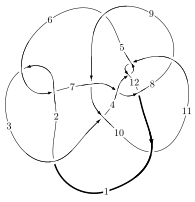
\includegraphics[width=112pt]{../../../GIT/diagram.site/Diagrams/png/1258_12a_0457.png}\\
\ \ \ A knot diagram\footnotemark}&
\allowdisplaybreaks
\textbf{Linearized knot diagam} \\
\cline{2-2}
 &
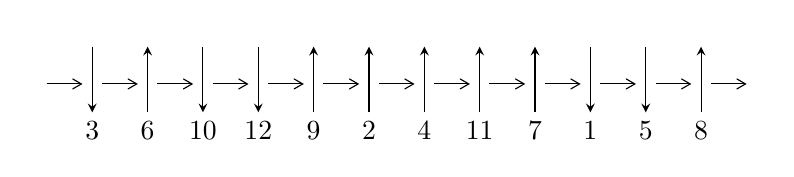
\begin{tikzpicture}[x=20pt, y=17pt]
	% nodes
	\node (C0) at (0, 0) {};
	\node (C1) at (1, 0) {};
	\node (C1U) at (1, +1) {};
	\node (C1D) at (1, -1) {3};

	\node (C2) at (2, 0) {};
	\node (C2U) at (2, +1) {};
	\node (C2D) at (2, -1) {6};

	\node (C3) at (3, 0) {};
	\node (C3U) at (3, +1) {};
	\node (C3D) at (3, -1) {10};

	\node (C4) at (4, 0) {};
	\node (C4U) at (4, +1) {};
	\node (C4D) at (4, -1) {12};

	\node (C5) at (5, 0) {};
	\node (C5U) at (5, +1) {};
	\node (C5D) at (5, -1) {9};

	\node (C6) at (6, 0) {};
	\node (C6U) at (6, +1) {};
	\node (C6D) at (6, -1) {2};

	\node (C7) at (7, 0) {};
	\node (C7U) at (7, +1) {};
	\node (C7D) at (7, -1) {4};

	\node (C8) at (8, 0) {};
	\node (C8U) at (8, +1) {};
	\node (C8D) at (8, -1) {11};

	\node (C9) at (9, 0) {};
	\node (C9U) at (9, +1) {};
	\node (C9D) at (9, -1) {7};

	\node (C10) at (10, 0) {};
	\node (C10U) at (10, +1) {};
	\node (C10D) at (10, -1) {1};

	\node (C11) at (11, 0) {};
	\node (C11U) at (11, +1) {};
	\node (C11D) at (11, -1) {5};

	\node (C12) at (12, 0) {};
	\node (C12U) at (12, +1) {};
	\node (C12D) at (12, -1) {8};
	\node (C13) at (13, 0) {};

	% arrows
	\draw[->,>={angle 60}]
	(C0) edge (C1) (C1) edge (C2) (C2) edge (C3) (C3) edge (C4) (C4) edge (C5) (C5) edge (C6) (C6) edge (C7) (C7) edge (C8) (C8) edge (C9) (C9) edge (C10) (C10) edge (C11) (C11) edge (C12) (C12) edge (C13) ;	\draw[->,>=stealth]
	(C1U) edge (C1D) (C2D) edge (C2U) (C3U) edge (C3D) (C4U) edge (C4D) (C5D) edge (C5U) (C6D) edge (C6U) (C7D) edge (C7U) (C8D) edge (C8U) (C9D) edge (C9U) (C10U) edge (C10D) (C11U) edge (C11D) (C12D) edge (C12U) ;
	\end{tikzpicture} \\
\hhline{~~} \\& 
\textbf{Solving Sequence} \\ \cline{2-2} 
 &
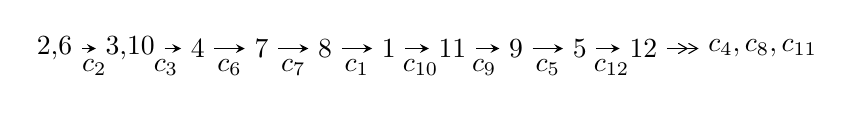
\begin{tikzpicture}[x=23pt, y=7pt]
	% node
	\node (A0) at (-1/8, 0) {2,6};
	\node (A1) at (17/16, 0) {3,10};
	\node (A2) at (17/8, 0) {4};
	\node (A3) at (25/8, 0) {7};
	\node (A4) at (33/8, 0) {8};
	\node (A5) at (41/8, 0) {1};
	\node (A6) at (49/8, 0) {11};
	\node (A7) at (57/8, 0) {9};
	\node (A8) at (65/8, 0) {5};
	\node (A9) at (73/8, 0) {12};
	\node (C1) at (1/2, -1) {$c_{2}$};
	\node (C2) at (13/8, -1) {$c_{3}$};
	\node (C3) at (21/8, -1) {$c_{6}$};
	\node (C4) at (29/8, -1) {$c_{7}$};
	\node (C5) at (37/8, -1) {$c_{1}$};
	\node (C6) at (45/8, -1) {$c_{10}$};
	\node (C7) at (53/8, -1) {$c_{9}$};
	\node (C8) at (61/8, -1) {$c_{5}$};
	\node (C9) at (69/8, -1) {$c_{12}$};
	\node (A10) at (11, 0) {$c_{4},c_{8},c_{11}$};

	% edge
	\draw[->,>=stealth]	
	(A0) edge (A1) (A1) edge (A2) (A2) edge (A3) (A3) edge (A4) (A4) edge (A5) (A5) edge (A6) (A6) edge (A7) (A7) edge (A8) (A8) edge (A9) ;
	\draw[->>,>={angle 60}]	
	(A9) edge (A10);
\end{tikzpicture} \\ 

\end{tabular} \\

\footnotetext{
The image of knot diagram is generated by the software ``\textbf{Draw programme}" developed by Andrew Bartholomew(\url{http://www.layer8.co.uk/maths/draw/index.htm\#Running-draw}), where we modified some parts for our purpose(\url{https://github.com/CATsTAILs/LinksPainter}).
}\phantom \\ \newline 
\centering \textbf{Ideals for irreducible components\footnotemark of $X_{\text{par}}$} 
 
\begin{align*}
I^u_{1}&=\langle 
1.58709\times10^{561} u^{181}+9.87432\times10^{561} u^{180}+\cdots+5.35199\times10^{561} b-9.54773\times10^{562},\\
\phantom{I^u_{1}}&\phantom{= \langle  }-1.66259\times10^{562} u^{181}-2.79221\times10^{562} u^{180}+\cdots+5.88719\times10^{562} a+3.00657\times10^{563},\\
\phantom{I^u_{1}}&\phantom{= \langle  }u^{182}- u^{181}+\cdots+195 u-11\rangle \\
I^u_{2}&=\langle 
-2.94627\times10^{21} u^{46}+1.06794\times10^{22} u^{45}+\cdots+2.90616\times10^{21} b-2.06732\times10^{22},\\
\phantom{I^u_{2}}&\phantom{= \langle  }-4.24175\times10^{21} u^{46}+1.09748\times10^{22} u^{45}+\cdots+2.90616\times10^{21} a-1.94328\times10^{22},\\
\phantom{I^u_{2}}&\phantom{= \langle  }u^{47}+13 u^{45}+\cdots+3 u-1\rangle \\
\\
\end{align*}
\raggedright * 2 irreducible components of $\dim_{\mathbb{C}}=0$, with total 229 representations.\\
\footnotetext{All coefficients of polynomials are rational numbers. But the coefficients are sometimes approximated in decimal forms when there is not enough margin.}
\newpage
\renewcommand{\arraystretch}{1}
\centering \section*{I. $I^u_{1}= \langle 1.59\times10^{561} u^{181}+9.87\times10^{561} u^{180}+\cdots+5.35\times10^{561} b-9.55\times10^{562},\;-1.66\times10^{562} u^{181}-2.79\times10^{562} u^{180}+\cdots+5.89\times10^{562} a+3.01\times10^{563},\;u^{182}- u^{181}+\cdots+195 u-11 \rangle$}
\flushleft \textbf{(i) Arc colorings}\\
\begin{tabular}{m{7pt} m{180pt} m{7pt} m{180pt} }
\flushright $a_{2}=$&$\begin{pmatrix}1\\0\end{pmatrix}$ \\
\flushright $a_{6}=$&$\begin{pmatrix}0\\u\end{pmatrix}$ \\
\flushright $a_{3}=$&$\begin{pmatrix}1\\- u^2\end{pmatrix}$ \\
\flushright $a_{10}=$&$\begin{pmatrix}0.282408 u^{181}+0.474286 u^{180}+\cdots-7.81834 u-5.10697\\-0.296542 u^{181}-1.84498 u^{180}+\cdots-292.837 u+17.8396\end{pmatrix}$ \\
\flushright $a_{4}=$&$\begin{pmatrix}0.426730 u^{181}+2.54621 u^{180}+\cdots+524.087 u-35.8491\\-0.183215 u^{181}+2.67594 u^{180}+\cdots+433.789 u-26.9732\end{pmatrix}$ \\
\flushright $a_{7}=$&$\begin{pmatrix}u\\u\end{pmatrix}$ \\
\flushright $a_{8}=$&$\begin{pmatrix}0.0954184 u^{181}+0.737891 u^{180}+\cdots+78.8011 u-1.90680\\-0.580714 u^{181}-0.712417 u^{180}+\cdots-101.183 u+7.71908\end{pmatrix}$ \\
\flushright $a_{1}=$&$\begin{pmatrix}u^2+1\\- u^4\end{pmatrix}$ \\
\flushright $a_{11}=$&$\begin{pmatrix}3.53650 u^{181}-3.37660 u^{180}+\cdots-747.932 u+37.4265\\3.15967 u^{181}-5.38431 u^{180}+\cdots-1000.45 u+57.9589\end{pmatrix}$ \\
\flushright $a_{9}=$&$\begin{pmatrix}2.86232 u^{181}-2.41148 u^{180}+\cdots-566.602 u+26.7734\\2.28337 u^{181}-4.73075 u^{180}+\cdots-851.621 u+49.7200\end{pmatrix}$ \\
\flushright $a_{5}=$&$\begin{pmatrix}-0.133531 u^{181}-1.04533 u^{180}+\cdots-355.789 u+27.2831\\1.09284 u^{181}-1.93033 u^{180}+\cdots-444.725 u+26.6777\end{pmatrix}$ \\
\flushright $a_{12}=$&$\begin{pmatrix}0.727233 u^{181}-1.06159 u^{180}+\cdots-360.131 u+18.9256\\0.934569 u^{181}-1.03798 u^{180}+\cdots-139.137 u+7.79370\end{pmatrix}$\\&\end{tabular}
\flushleft \textbf{(ii) Obstruction class $= -1$}\\~\\
\flushleft \textbf{(iii) Cusp Shapes $= -1.66160 u^{181}-0.329436 u^{180}+\cdots+113.796 u-4.78638$}\\~\\
\newpage\renewcommand{\arraystretch}{1}
\flushleft \textbf{(iv) u-Polynomials at the component}\newline \\
\begin{tabular}{m{50pt}|m{274pt}}
Crossings & \hspace{64pt}u-Polynomials at each crossing \\
\hline $$\begin{aligned}c_{1}\end{aligned}$$&$\begin{aligned}
&u^{182}+77 u^{181}+\cdots+8263 u+121
\end{aligned}$\\
\hline $$\begin{aligned}c_{2},c_{6}\end{aligned}$$&$\begin{aligned}
&u^{182}- u^{181}+\cdots+195 u-11
\end{aligned}$\\
\hline $$\begin{aligned}c_{3}\end{aligned}$$&$\begin{aligned}
&u^{182}+2 u^{181}+\cdots-5309082 u-451273
\end{aligned}$\\
\hline $$\begin{aligned}c_{4},c_{11}\end{aligned}$$&$\begin{aligned}
&u^{182}+2 u^{181}+\cdots+19 u-1
\end{aligned}$\\
\hline $$\begin{aligned}c_{5}\end{aligned}$$&$\begin{aligned}
&u^{182}+2 u^{181}+\cdots-38159038193725 u-9874199002121
\end{aligned}$\\
\hline $$\begin{aligned}c_{7}\end{aligned}$$&$\begin{aligned}
&u^{182}-3 u^{181}+\cdots-16973493258 u+2170070627
\end{aligned}$\\
\hline $$\begin{aligned}c_{8}\end{aligned}$$&$\begin{aligned}
&u^{182}-13 u^{181}+\cdots-32599410 u+3488929
\end{aligned}$\\
\hline $$\begin{aligned}c_{9}\end{aligned}$$&$\begin{aligned}
&u^{182}-8 u^{181}+\cdots+120499307 u-33795031
\end{aligned}$\\
\hline $$\begin{aligned}c_{10}\end{aligned}$$&$\begin{aligned}
&u^{182}-16 u^{181}+\cdots+87245097403 u-3309477077
\end{aligned}$\\
\hline $$\begin{aligned}c_{12}\end{aligned}$$&$\begin{aligned}
&u^{182}+u^{181}+\cdots+38826485 u+8693093
\end{aligned}$\\
\hline
\end{tabular}\\~\\
\newpage\renewcommand{\arraystretch}{1}
\flushleft \textbf{(v) Riley Polynomials at the component}\newline \\
\begin{tabular}{m{50pt}|m{274pt}}
Crossings & \hspace{64pt}Riley Polynomials at each crossing \\
\hline $$\begin{aligned}c_{1}\end{aligned}$$&$\begin{aligned}
&y^{182}+69 y^{181}+\cdots+304853435 y+14641
\end{aligned}$\\
\hline $$\begin{aligned}c_{2},c_{6}\end{aligned}$$&$\begin{aligned}
&y^{182}+77 y^{181}+\cdots+8263 y+121
\end{aligned}$\\
\hline $$\begin{aligned}c_{3}\end{aligned}$$&$\begin{aligned}
&y^{182}+44 y^{181}+\cdots-374808253700 y+203647320529
\end{aligned}$\\
\hline $$\begin{aligned}c_{4},c_{11}\end{aligned}$$&$\begin{aligned}
&y^{182}+126 y^{181}+\cdots-113 y+1
\end{aligned}$\\
\hline $$\begin{aligned}c_{5}\end{aligned}$$&$\begin{aligned}
&y^{182}-100 y^{181}+\cdots-6.27\times10^{27} y+9.75\times10^{25}
\end{aligned}$\\
\hline $$\begin{aligned}c_{7}\end{aligned}$$&$\begin{aligned}
&y^{182}-83 y^{181}+\cdots+7.07\times10^{20} y+4.71\times10^{18}
\end{aligned}$\\
\hline $$\begin{aligned}c_{8}\end{aligned}$$&$\begin{aligned}
&y^{182}-65 y^{181}+\cdots+5327570686683198 y+12172625567041
\end{aligned}$\\
\hline $$\begin{aligned}c_{9}\end{aligned}$$&$\begin{aligned}
&y^{182}-60 y^{181}+\cdots-84230223266656641 y+1142104120290961
\end{aligned}$\\
\hline $$\begin{aligned}c_{10}\end{aligned}$$&$\begin{aligned}
&y^{182}+70 y^{181}+\cdots-5.83\times10^{20} y+1.10\times10^{19}
\end{aligned}$\\
\hline $$\begin{aligned}c_{12}\end{aligned}$$&$\begin{aligned}
&y^{182}-57 y^{181}+\cdots-3145101509628851 y+75569865906649
\end{aligned}$\\
\hline
\end{tabular}\\~\\
\newpage\flushleft \textbf{(vi) Complex Volumes and Cusp Shapes}
$$\begin{array}{c|c|c}  
\text{Solutions to }I^u_{1}& \I (\text{vol} + \sqrt{-1}CS) & \text{Cusp shape}\\
 \hline 
\begin{aligned}
u &= \phantom{-}0.631933 + 0.776970 I \\
a &= -1.65261 - 1.75545 I \\
b &= -1.74171 + 0.24098 I\end{aligned}
 & \phantom{-}6.97272 - 0.23557 I & \phantom{-0.000000 } 0 \\ \hline\begin{aligned}
u &= \phantom{-}0.631933 - 0.776970 I \\
a &= -1.65261 + 1.75545 I \\
b &= -1.74171 - 0.24098 I\end{aligned}
 & \phantom{-}6.97272 + 0.23557 I & \phantom{-0.000000 } 0 \\ \hline\begin{aligned}
u &= -0.632760 + 0.770322 I \\
a &= -0.11056 + 2.39938 I \\
b &= -0.34857 + 1.45255 I\end{aligned}
 & \phantom{-}7.91436 + 5.68837 I & \phantom{-0.000000 } 0 \\ \hline\begin{aligned}
u &= -0.632760 - 0.770322 I \\
a &= -0.11056 - 2.39938 I \\
b &= -0.34857 - 1.45255 I\end{aligned}
 & \phantom{-}7.91436 - 5.68837 I & \phantom{-0.000000 } 0 \\ \hline\begin{aligned}
u &= -0.505651 + 0.867835 I \\
a &= \phantom{-}0.20529 - 2.28170 I \\
b &= \phantom{-}1.57861 - 2.01284 I\end{aligned}
 & \phantom{-}2.46270 - 5.69294 I & \phantom{-0.000000 } 0 \\ \hline\begin{aligned}
u &= -0.505651 - 0.867835 I \\
a &= \phantom{-}0.20529 + 2.28170 I \\
b &= \phantom{-}1.57861 + 2.01284 I\end{aligned}
 & \phantom{-}2.46270 + 5.69294 I & \phantom{-0.000000 } 0 \\ \hline\begin{aligned}
u &= \phantom{-}0.555676 + 0.856464 I \\
a &= -0.373690 + 0.189044 I \\
b &= -1.375140 - 0.038000 I\end{aligned}
 & \phantom{-}0.73313 + 1.72700 I & \phantom{-0.000000 } 0 \\ \hline\begin{aligned}
u &= \phantom{-}0.555676 - 0.856464 I \\
a &= -0.373690 - 0.189044 I \\
b &= -1.375140 + 0.038000 I\end{aligned}
 & \phantom{-}0.73313 - 1.72700 I & \phantom{-0.000000 } 0 \\ \hline\begin{aligned}
u &= \phantom{-}0.553470 + 0.860165 I \\
a &= -0.42398 - 1.46537 I \\
b &= -0.057580 - 0.315865 I\end{aligned}
 & \phantom{-}0.72308 + 2.71161 I & \phantom{-0.000000 } 0 \\ \hline\begin{aligned}
u &= \phantom{-}0.553470 - 0.860165 I \\
a &= -0.42398 + 1.46537 I \\
b &= -0.057580 + 0.315865 I\end{aligned}
 & \phantom{-}0.72308 - 2.71161 I & \phantom{-0.000000 } 0\\
 \hline 
 \end{array}$$\newpage$$\begin{array}{c|c|c}  
\text{Solutions to }I^u_{1}& \I (\text{vol} + \sqrt{-1}CS) & \text{Cusp shape}\\
 \hline 
\begin{aligned}
u &= -0.632870 + 0.807341 I \\
a &= \phantom{-}1.37911 - 1.32103 I \\
b &= \phantom{-}1.48733 + 0.40353 I\end{aligned}
 & \phantom{-}3.51581 - 0.69080 I & \phantom{-0.000000 } 0 \\ \hline\begin{aligned}
u &= -0.632870 - 0.807341 I \\
a &= \phantom{-}1.37911 + 1.32103 I \\
b &= \phantom{-}1.48733 - 0.40353 I\end{aligned}
 & \phantom{-}3.51581 + 0.69080 I & \phantom{-0.000000 } 0 \\ \hline\begin{aligned}
u &= \phantom{-}0.634227 + 0.807382 I \\
a &= -0.75123 + 1.66878 I \\
b &= \phantom{-}1.83427 + 1.96031 I\end{aligned}
 & \phantom{-}7.79532 - 4.87002 I & \phantom{-0.000000 } 0 \\ \hline\begin{aligned}
u &= \phantom{-}0.634227 - 0.807382 I \\
a &= -0.75123 - 1.66878 I \\
b &= \phantom{-}1.83427 - 1.96031 I\end{aligned}
 & \phantom{-}7.79532 + 4.87002 I & \phantom{-0.000000 } 0 \\ \hline\begin{aligned}
u &= \phantom{-}0.243407 + 1.001150 I \\
a &= \phantom{-}0.530592 - 1.034200 I \\
b &= \phantom{-}1.145160 - 0.367665 I\end{aligned}
 & -1.57699 - 0.96008 I & \phantom{-0.000000 } 0 \\ \hline\begin{aligned}
u &= \phantom{-}0.243407 - 1.001150 I \\
a &= \phantom{-}0.530592 + 1.034200 I \\
b &= \phantom{-}1.145160 + 0.367665 I\end{aligned}
 & -1.57699 + 0.96008 I & \phantom{-0.000000 } 0 \\ \hline\begin{aligned}
u &= -0.916874 + 0.471952 I \\
a &= -0.002829 + 1.150230 I \\
b &= -0.754882 + 0.535498 I\end{aligned}
 & \phantom{-}9.47112 + 2.17209 I & \phantom{-0.000000 } 0 \\ \hline\begin{aligned}
u &= -0.916874 - 0.471952 I \\
a &= -0.002829 - 1.150230 I \\
b &= -0.754882 - 0.535498 I\end{aligned}
 & \phantom{-}9.47112 - 2.17209 I & \phantom{-0.000000 } 0 \\ \hline\begin{aligned}
u &= \phantom{-}0.892126 + 0.527577 I \\
a &= \phantom{-}0.659159 + 1.114030 I \\
b &= \phantom{-}1.63494 + 0.05175 I\end{aligned}
 & \phantom{-}9.85070 - 2.32266 I & \phantom{-0.000000 } 0 \\ \hline\begin{aligned}
u &= \phantom{-}0.892126 - 0.527577 I \\
a &= \phantom{-}0.659159 - 1.114030 I \\
b &= \phantom{-}1.63494 - 0.05175 I\end{aligned}
 & \phantom{-}9.85070 + 2.32266 I & \phantom{-0.000000 } 0\\
 \hline 
 \end{array}$$\newpage$$\begin{array}{c|c|c}  
\text{Solutions to }I^u_{1}& \I (\text{vol} + \sqrt{-1}CS) & \text{Cusp shape}\\
 \hline 
\begin{aligned}
u &= -0.663555 + 0.797112 I \\
a &= \phantom{-}1.33810 - 0.99347 I \\
b &= \phantom{-}2.29960 - 0.27379 I\end{aligned}
 & \phantom{-}7.55519 - 0.30516 I & \phantom{-0.000000 } 0 \\ \hline\begin{aligned}
u &= -0.663555 - 0.797112 I \\
a &= \phantom{-}1.33810 + 0.99347 I \\
b &= \phantom{-}2.29960 + 0.27379 I\end{aligned}
 & \phantom{-}7.55519 + 0.30516 I & \phantom{-0.000000 } 0 \\ \hline\begin{aligned}
u &= \phantom{-}0.650144 + 0.815932 I \\
a &= \phantom{-}0.30077 + 2.29042 I \\
b &= \phantom{-}0.63200 + 1.61924 I\end{aligned}
 & \phantom{-}3.47733 + 0.38218 I & \phantom{-0.000000 } 0 \\ \hline\begin{aligned}
u &= \phantom{-}0.650144 - 0.815932 I \\
a &= \phantom{-}0.30077 - 2.29042 I \\
b &= \phantom{-}0.63200 - 1.61924 I\end{aligned}
 & \phantom{-}3.47733 - 0.38218 I & \phantom{-0.000000 } 0 \\ \hline\begin{aligned}
u &= -0.874669 + 0.580375 I \\
a &= \phantom{-}0.92398 - 1.08793 I \\
b &= \phantom{-}1.371120 + 0.193415 I\end{aligned}
 & \phantom{-}4.85248 + 3.78665 I & \phantom{-0.000000 } 0 \\ \hline\begin{aligned}
u &= -0.874669 - 0.580375 I \\
a &= \phantom{-}0.92398 + 1.08793 I \\
b &= \phantom{-}1.371120 - 0.193415 I\end{aligned}
 & \phantom{-}4.85248 - 3.78665 I & \phantom{-0.000000 } 0 \\ \hline\begin{aligned}
u &= -0.458613 + 0.830611 I \\
a &= \phantom{-}1.86473 - 0.59837 I \\
b &= \phantom{-}1.59506 + 0.41043 I\end{aligned}
 & \phantom{-}2.58944 + 1.69215 I & \phantom{-0.000000 } 0 \\ \hline\begin{aligned}
u &= -0.458613 - 0.830611 I \\
a &= \phantom{-}1.86473 + 0.59837 I \\
b &= \phantom{-}1.59506 - 0.41043 I\end{aligned}
 & \phantom{-}2.58944 - 1.69215 I & \phantom{-0.000000 } 0 \\ \hline\begin{aligned}
u &= \phantom{-}0.933388 + 0.497942 I \\
a &= -0.58218 - 1.36147 I \\
b &= -1.320980 + 0.133542 I\end{aligned}
 & \phantom{-}8.58940 - 4.72156 I & \phantom{-0.000000 } 0 \\ \hline\begin{aligned}
u &= \phantom{-}0.933388 - 0.497942 I \\
a &= -0.58218 + 1.36147 I \\
b &= -1.320980 - 0.133542 I\end{aligned}
 & \phantom{-}8.58940 + 4.72156 I & \phantom{-0.000000 } 0\\
 \hline 
 \end{array}$$\newpage$$\begin{array}{c|c|c}  
\text{Solutions to }I^u_{1}& \I (\text{vol} + \sqrt{-1}CS) & \text{Cusp shape}\\
 \hline 
\begin{aligned}
u &= -0.924489 + 0.526819 I \\
a &= -0.810217 + 1.092250 I \\
b &= -1.51468 - 0.11098 I\end{aligned}
 & \phantom{-}5.51807 + 8.96111 I & \phantom{-0.000000 } 0 \\ \hline\begin{aligned}
u &= -0.924489 - 0.526819 I \\
a &= -0.810217 - 1.092250 I \\
b &= -1.51468 + 0.11098 I\end{aligned}
 & \phantom{-}5.51807 - 8.96111 I & \phantom{-0.000000 } 0 \\ \hline\begin{aligned}
u &= -0.912357 + 0.549512 I \\
a &= -0.065292 - 1.069180 I \\
b &= \phantom{-}1.240240 - 0.453768 I\end{aligned}
 & \phantom{-}8.94932 + 0.14223 I & \phantom{-0.000000 } 0 \\ \hline\begin{aligned}
u &= -0.912357 - 0.549512 I \\
a &= -0.065292 + 1.069180 I \\
b &= \phantom{-}1.240240 + 0.453768 I\end{aligned}
 & \phantom{-}8.94932 - 0.14223 I & \phantom{-0.000000 } 0 \\ \hline\begin{aligned}
u &= -0.465535 + 0.809704 I \\
a &= \phantom{-}0.169775 + 0.018988 I \\
b &= -0.944350 + 1.000900 I\end{aligned}
 & \phantom{-}2.10752 + 1.81777 I & \phantom{-0.000000 } 0 \\ \hline\begin{aligned}
u &= -0.465535 - 0.809704 I \\
a &= \phantom{-}0.169775 - 0.018988 I \\
b &= -0.944350 - 1.000900 I\end{aligned}
 & \phantom{-}2.10752 - 1.81777 I & \phantom{-0.000000 } 0 \\ \hline\begin{aligned}
u &= -0.626727 + 0.872915 I \\
a &= \phantom{-}0.07240 - 1.54884 I \\
b &= \phantom{-}1.76358 - 1.45067 I\end{aligned}
 & \phantom{-}3.31560 - 4.24542 I & \phantom{-0.000000 } 0 \\ \hline\begin{aligned}
u &= -0.626727 - 0.872915 I \\
a &= \phantom{-}0.07240 + 1.54884 I \\
b &= \phantom{-}1.76358 + 1.45067 I\end{aligned}
 & \phantom{-}3.31560 + 4.24542 I & \phantom{-0.000000 } 0 \\ \hline\begin{aligned}
u &= \phantom{-}0.452245 + 0.805252 I \\
a &= \phantom{-}0.517112 + 1.097860 I \\
b &= \phantom{-}0.834423 + 0.856549 I\end{aligned}
 & -0.02246 + 1.79724 I & \phantom{-0.000000 } 0 \\ \hline\begin{aligned}
u &= \phantom{-}0.452245 - 0.805252 I \\
a &= \phantom{-}0.517112 - 1.097860 I \\
b &= \phantom{-}0.834423 - 0.856549 I\end{aligned}
 & -0.02246 - 1.79724 I & \phantom{-0.000000 } 0\\
 \hline 
 \end{array}$$\newpage$$\begin{array}{c|c|c}  
\text{Solutions to }I^u_{1}& \I (\text{vol} + \sqrt{-1}CS) & \text{Cusp shape}\\
 \hline 
\begin{aligned}
u &= \phantom{-}0.220942 + 1.055330 I \\
a &= \phantom{-}1.369150 + 0.012423 I \\
b &= \phantom{-}0.549632 - 1.178900 I\end{aligned}
 & \phantom{-}1.95420 - 4.55320 I & \phantom{-0.000000 } 0 \\ \hline\begin{aligned}
u &= \phantom{-}0.220942 - 1.055330 I \\
a &= \phantom{-}1.369150 - 0.012423 I \\
b &= \phantom{-}0.549632 + 1.178900 I\end{aligned}
 & \phantom{-}1.95420 + 4.55320 I & \phantom{-0.000000 } 0 \\ \hline\begin{aligned}
u &= \phantom{-}0.637383 + 0.870473 I \\
a &= \phantom{-}1.86831 + 0.16044 I \\
b &= \phantom{-}2.33244 - 0.08278 I\end{aligned}
 & \phantom{-}3.31211 + 4.63591 I & \phantom{-0.000000 } 0 \\ \hline\begin{aligned}
u &= \phantom{-}0.637383 - 0.870473 I \\
a &= \phantom{-}1.86831 - 0.16044 I \\
b &= \phantom{-}2.33244 + 0.08278 I\end{aligned}
 & \phantom{-}3.31211 - 4.63591 I & \phantom{-0.000000 } 0 \\ \hline\begin{aligned}
u &= \phantom{-}0.937825 + 0.534651 I \\
a &= \phantom{-}0.87212 + 1.15341 I \\
b &= \phantom{-}1.55379 - 0.24257 I\end{aligned}
 & \phantom{-}10.2706 - 14.8755 I & \phantom{-0.000000 } 0 \\ \hline\begin{aligned}
u &= \phantom{-}0.937825 - 0.534651 I \\
a &= \phantom{-}0.87212 - 1.15341 I \\
b &= \phantom{-}1.55379 + 0.24257 I\end{aligned}
 & \phantom{-}10.2706 + 14.8755 I & \phantom{-0.000000 } 0 \\ \hline\begin{aligned}
u &= -0.708071 + 0.815604 I \\
a &= -0.10069 + 1.94194 I \\
b &= -0.70412 + 1.32099 I\end{aligned}
 & \phantom{-}8.20130 - 6.30272 I & \phantom{-0.000000 } 0 \\ \hline\begin{aligned}
u &= -0.708071 - 0.815604 I \\
a &= -0.10069 - 1.94194 I \\
b &= -0.70412 - 1.32099 I\end{aligned}
 & \phantom{-}8.20130 + 6.30272 I & \phantom{-0.000000 } 0 \\ \hline\begin{aligned}
u &= \phantom{-}0.441114 + 0.807249 I \\
a &= -0.19134 - 2.42815 I \\
b &= -0.91796 - 1.43722 I\end{aligned}
 & -0.022971 + 0.996096 I & \phantom{-0.000000 } 0 \\ \hline\begin{aligned}
u &= \phantom{-}0.441114 - 0.807249 I \\
a &= -0.19134 + 2.42815 I \\
b &= -0.91796 + 1.43722 I\end{aligned}
 & -0.022971 - 0.996096 I & \phantom{-0.000000 } 0\\
 \hline 
 \end{array}$$\newpage$$\begin{array}{c|c|c}  
\text{Solutions to }I^u_{1}& \I (\text{vol} + \sqrt{-1}CS) & \text{Cusp shape}\\
 \hline 
\begin{aligned}
u &= \phantom{-}0.622855 + 0.886369 I \\
a &= \phantom{-}2.24095 + 1.13511 I \\
b &= \phantom{-}1.81291 - 1.50251 I\end{aligned}
 & \phantom{-}7.55009 + 9.79273 I & \phantom{-0.000000 } 0 \\ \hline\begin{aligned}
u &= \phantom{-}0.622855 - 0.886369 I \\
a &= \phantom{-}2.24095 - 1.13511 I \\
b &= \phantom{-}1.81291 + 1.50251 I\end{aligned}
 & \phantom{-}7.55009 - 9.79273 I & \phantom{-0.000000 } 0 \\ \hline\begin{aligned}
u &= -0.530823 + 0.745021 I \\
a &= \phantom{-}0.502174 + 0.555666 I \\
b &= -0.97541 + 1.32446 I\end{aligned}
 & \phantom{-}1.95963 + 1.72495 I & \phantom{-0.000000 } 0 \\ \hline\begin{aligned}
u &= -0.530823 - 0.745021 I \\
a &= \phantom{-}0.502174 - 0.555666 I \\
b &= -0.97541 - 1.32446 I\end{aligned}
 & \phantom{-}1.95963 - 1.72495 I & \phantom{-0.000000 } 0 \\ \hline\begin{aligned}
u &= -0.160219 + 0.897897 I \\
a &= -0.901106 - 0.170529 I \\
b &= \phantom{-}0.453433 + 0.217919 I\end{aligned}
 & \phantom{-}1.35572 - 4.86438 I & \phantom{-0.000000 } 0 \\ \hline\begin{aligned}
u &= -0.160219 - 0.897897 I \\
a &= -0.901106 + 0.170529 I \\
b &= \phantom{-}0.453433 - 0.217919 I\end{aligned}
 & \phantom{-}1.35572 + 4.86438 I & \phantom{-0.000000 } 0 \\ \hline\begin{aligned}
u &= -0.571472 + 0.927694 I \\
a &= -1.298200 + 0.399511 I \\
b &= -0.382575 - 0.835713 I\end{aligned}
 & \phantom{-}1.36817 - 6.19695 I & \phantom{-0.000000 } 0 \\ \hline\begin{aligned}
u &= -0.571472 - 0.927694 I \\
a &= -1.298200 - 0.399511 I \\
b &= -0.382575 + 0.835713 I\end{aligned}
 & \phantom{-}1.36817 + 6.19695 I & \phantom{-0.000000 } 0 \\ \hline\begin{aligned}
u &= \phantom{-}0.467156 + 0.986445 I \\
a &= -0.852742 - 0.656440 I \\
b &= -1.53925 - 0.07375 I\end{aligned}
 & -0.67167 + 2.67554 I & \phantom{-0.000000 } 0 \\ \hline\begin{aligned}
u &= \phantom{-}0.467156 - 0.986445 I \\
a &= -0.852742 + 0.656440 I \\
b &= -1.53925 + 0.07375 I\end{aligned}
 & -0.67167 - 2.67554 I & \phantom{-0.000000 } 0\\
 \hline 
 \end{array}$$\newpage$$\begin{array}{c|c|c}  
\text{Solutions to }I^u_{1}& \I (\text{vol} + \sqrt{-1}CS) & \text{Cusp shape}\\
 \hline 
\begin{aligned}
u &= \phantom{-}0.973048 + 0.519295 I \\
a &= \phantom{-}0.014391 + 0.866018 I \\
b &= \phantom{-}0.755408 + 0.484817 I\end{aligned}
 & \phantom{-}5.32052 + 3.86352 I & \phantom{-0.000000 } 0 \\ \hline\begin{aligned}
u &= \phantom{-}0.973048 - 0.519295 I \\
a &= \phantom{-}0.014391 - 0.866018 I \\
b &= \phantom{-}0.755408 - 0.484817 I\end{aligned}
 & \phantom{-}5.32052 - 3.86352 I & \phantom{-0.000000 } 0 \\ \hline\begin{aligned}
u &= \phantom{-}0.854993 + 0.697740 I \\
a &= -1.31960 - 0.90738 I \\
b &= -1.73895 + 0.52611 I\end{aligned}
 & \phantom{-}8.01369 - 4.13820 I & \phantom{-0.000000 } 0 \\ \hline\begin{aligned}
u &= \phantom{-}0.854993 - 0.697740 I \\
a &= -1.31960 + 0.90738 I \\
b &= -1.73895 - 0.52611 I\end{aligned}
 & \phantom{-}8.01369 + 4.13820 I & \phantom{-0.000000 } 0 \\ \hline\begin{aligned}
u &= \phantom{-}0.733957 + 0.824303 I \\
a &= \phantom{-}0.290309 - 1.384090 I \\
b &= -1.54739 - 1.37090 I\end{aligned}
 & \phantom{-}7.38312 + 5.08653 I & \phantom{-0.000000 } 0 \\ \hline\begin{aligned}
u &= \phantom{-}0.733957 - 0.824303 I \\
a &= \phantom{-}0.290309 + 1.384090 I \\
b &= -1.54739 + 1.37090 I\end{aligned}
 & \phantom{-}7.38312 - 5.08653 I & \phantom{-0.000000 } 0 \\ \hline\begin{aligned}
u &= -0.646203 + 0.895156 I \\
a &= \phantom{-}0.94098 - 2.16469 I \\
b &= \phantom{-}1.63609 - 0.98694 I\end{aligned}
 & \phantom{-}7.25316 - 4.78011 I & \phantom{-0.000000 } 0 \\ \hline\begin{aligned}
u &= -0.646203 - 0.895156 I \\
a &= \phantom{-}0.94098 + 2.16469 I \\
b &= \phantom{-}1.63609 + 0.98694 I\end{aligned}
 & \phantom{-}7.25316 + 4.78011 I & \phantom{-0.000000 } 0 \\ \hline\begin{aligned}
u &= \phantom{-}0.622702 + 0.911924 I \\
a &= -0.56426 - 1.60083 I \\
b &= -2.29930 - 1.39669 I\end{aligned}
 & \phantom{-}6.55259 + 5.15491 I & \phantom{-0.000000 } 0 \\ \hline\begin{aligned}
u &= \phantom{-}0.622702 - 0.911924 I \\
a &= -0.56426 + 1.60083 I \\
b &= -2.29930 + 1.39669 I\end{aligned}
 & \phantom{-}6.55259 - 5.15491 I & \phantom{-0.000000 } 0\\
 \hline 
 \end{array}$$\newpage$$\begin{array}{c|c|c}  
\text{Solutions to }I^u_{1}& \I (\text{vol} + \sqrt{-1}CS) & \text{Cusp shape}\\
 \hline 
\begin{aligned}
u &= -0.625395 + 0.915387 I \\
a &= -1.72882 - 0.21541 I \\
b &= -2.36328 - 0.43256 I\end{aligned}
 & \phantom{-}7.46437 - 10.62170 I & \phantom{-0.000000 } 0 \\ \hline\begin{aligned}
u &= -0.625395 - 0.915387 I \\
a &= -1.72882 + 0.21541 I \\
b &= -2.36328 + 0.43256 I\end{aligned}
 & \phantom{-}7.46437 + 10.62170 I & \phantom{-0.000000 } 0 \\ \hline\begin{aligned}
u &= \phantom{-}0.086041 + 1.105460 I \\
a &= \phantom{-}0.149188 - 0.169317 I \\
b &= -0.644765 + 0.259046 I\end{aligned}
 & -1.74919 + 2.67650 I & \phantom{-0.000000 } 0 \\ \hline\begin{aligned}
u &= \phantom{-}0.086041 - 1.105460 I \\
a &= \phantom{-}0.149188 + 0.169317 I \\
b &= -0.644765 - 0.259046 I\end{aligned}
 & -1.74919 - 2.67650 I & \phantom{-0.000000 } 0 \\ \hline\begin{aligned}
u &= \phantom{-}0.146549 + 1.101730 I \\
a &= -0.094814 + 0.750696 I \\
b &= -0.701831 + 0.844087 I\end{aligned}
 & -1.22941 + 1.28711 I & \phantom{-0.000000 } 0 \\ \hline\begin{aligned}
u &= \phantom{-}0.146549 - 1.101730 I \\
a &= -0.094814 - 0.750696 I \\
b &= -0.701831 - 0.844087 I\end{aligned}
 & -1.22941 - 1.28711 I & \phantom{-0.000000 } 0 \\ \hline\begin{aligned}
u &= \phantom{-}0.728249 + 0.850972 I \\
a &= -1.19782 - 1.01054 I \\
b &= -1.45992 + 0.72846 I\end{aligned}
 & \phantom{-}7.30499 + 0.45145 I & \phantom{-0.000000 } 0 \\ \hline\begin{aligned}
u &= \phantom{-}0.728249 - 0.850972 I \\
a &= -1.19782 + 1.01054 I \\
b &= -1.45992 - 0.72846 I\end{aligned}
 & \phantom{-}7.30499 - 0.45145 I & \phantom{-0.000000 } 0 \\ \hline\begin{aligned}
u &= -0.170408 + 1.111120 I \\
a &= -0.518963 + 0.268132 I \\
b &= \phantom{-}0.232205 - 0.164738 I\end{aligned}
 & -5.42453 - 0.61915 I & \phantom{-0.000000 } 0 \\ \hline\begin{aligned}
u &= -0.170408 - 1.111120 I \\
a &= -0.518963 - 0.268132 I \\
b &= \phantom{-}0.232205 + 0.164738 I\end{aligned}
 & -5.42453 + 0.61915 I & \phantom{-0.000000 } 0\\
 \hline 
 \end{array}$$\newpage$$\begin{array}{c|c|c}  
\text{Solutions to }I^u_{1}& \I (\text{vol} + \sqrt{-1}CS) & \text{Cusp shape}\\
 \hline 
\begin{aligned}
u &= -0.713965 + 0.869974 I \\
a &= -1.333890 + 0.188730 I \\
b &= -1.74912 - 0.20946 I\end{aligned}
 & \phantom{-}8.04336 + 0.87793 I & \phantom{-0.000000 } 0 \\ \hline\begin{aligned}
u &= -0.713965 - 0.869974 I \\
a &= -1.333890 - 0.188730 I \\
b &= -1.74912 + 0.20946 I\end{aligned}
 & \phantom{-}8.04336 - 0.87793 I & \phantom{-0.000000 } 0 \\ \hline\begin{aligned}
u &= -0.203912 + 0.850305 I \\
a &= \phantom{-}0.21411 + 1.85695 I \\
b &= -0.88888 + 1.25171 I\end{aligned}
 & -0.65134 + 1.63840 I & \phantom{-0.000000 } 0 \\ \hline\begin{aligned}
u &= -0.203912 - 0.850305 I \\
a &= \phantom{-}0.21411 - 1.85695 I \\
b &= -0.88888 - 1.25171 I\end{aligned}
 & -0.65134 - 1.63840 I & \phantom{-0.000000 } 0 \\ \hline\begin{aligned}
u &= -1.013160 + 0.496296 I \\
a &= \phantom{-}0.173474 + 0.797453 I \\
b &= -0.726329 + 0.525125 I\end{aligned}
 & \phantom{-}9.87586 - 9.51235 I & \phantom{-0.000000 } 0 \\ \hline\begin{aligned}
u &= -1.013160 - 0.496296 I \\
a &= \phantom{-}0.173474 - 0.797453 I \\
b &= -0.726329 - 0.525125 I\end{aligned}
 & \phantom{-}9.87586 + 9.51235 I & \phantom{-0.000000 } 0 \\ \hline\begin{aligned}
u &= -0.509438 + 1.010740 I \\
a &= -0.657047 + 0.822412 I \\
b &= -0.174623 + 0.531939 I\end{aligned}
 & \phantom{-}1.34232 - 5.62268 I & \phantom{-0.000000 } 0 \\ \hline\begin{aligned}
u &= -0.509438 - 1.010740 I \\
a &= -0.657047 - 0.822412 I \\
b &= -0.174623 - 0.531939 I\end{aligned}
 & \phantom{-}1.34232 + 5.62268 I & \phantom{-0.000000 } 0 \\ \hline\begin{aligned}
u &= \phantom{-}0.194485 + 1.115360 I \\
a &= \phantom{-}0.350100 + 0.186108 I \\
b &= -0.608444 - 0.027519 I\end{aligned}
 & -3.11951 + 4.78627 I & \phantom{-0.000000 } 0 \\ \hline\begin{aligned}
u &= \phantom{-}0.194485 - 1.115360 I \\
a &= \phantom{-}0.350100 - 0.186108 I \\
b &= -0.608444 + 0.027519 I\end{aligned}
 & -3.11951 - 4.78627 I & \phantom{-0.000000 } 0\\
 \hline 
 \end{array}$$\newpage$$\begin{array}{c|c|c}  
\text{Solutions to }I^u_{1}& \I (\text{vol} + \sqrt{-1}CS) & \text{Cusp shape}\\
 \hline 
\begin{aligned}
u &= \phantom{-}0.577569 + 0.986336 I \\
a &= -1.30379 - 2.11625 I \\
b &= -1.95283 - 1.76243 I\end{aligned}
 & \phantom{-}0.52117 + 6.74313 I & \phantom{-0.000000 } 0 \\ \hline\begin{aligned}
u &= \phantom{-}0.577569 - 0.986336 I \\
a &= -1.30379 + 2.11625 I \\
b &= -1.95283 + 1.76243 I\end{aligned}
 & \phantom{-}0.52117 - 6.74313 I & \phantom{-0.000000 } 0 \\ \hline\begin{aligned}
u &= \phantom{-}0.539310 + 1.017660 I \\
a &= \phantom{-}0.48284 + 1.45251 I \\
b &= \phantom{-}1.21063 + 1.31370 I\end{aligned}
 & -1.04203 + 1.94035 I & \phantom{-0.000000 } 0 \\ \hline\begin{aligned}
u &= \phantom{-}0.539310 - 1.017660 I \\
a &= \phantom{-}0.48284 - 1.45251 I \\
b &= \phantom{-}1.21063 - 1.31370 I\end{aligned}
 & -1.04203 - 1.94035 I & \phantom{-0.000000 } 0 \\ \hline\begin{aligned}
u &= -0.674362 + 0.513171 I \\
a &= \phantom{-}0.217297 - 1.068620 I \\
b &= \phantom{-}0.480136 + 0.394938 I\end{aligned}
 & \phantom{-}4.23188 + 1.98085 I & \phantom{-0.000000 } 0 \\ \hline\begin{aligned}
u &= -0.674362 - 0.513171 I \\
a &= \phantom{-}0.217297 + 1.068620 I \\
b &= \phantom{-}0.480136 - 0.394938 I\end{aligned}
 & \phantom{-}4.23188 - 1.98085 I & \phantom{-0.000000 } 0 \\ \hline\begin{aligned}
u &= \phantom{-}0.523596 + 0.665424 I \\
a &= -1.93350 - 1.53251 I \\
b &= -2.02164 - 0.92803 I\end{aligned}
 & \phantom{-}1.55166 - 2.20765 I & \phantom{-0.000000 } 0 \\ \hline\begin{aligned}
u &= \phantom{-}0.523596 - 0.665424 I \\
a &= -1.93350 + 1.53251 I \\
b &= -2.02164 + 0.92803 I\end{aligned}
 & \phantom{-}1.55166 + 2.20765 I & \phantom{-0.000000 } 0 \\ \hline\begin{aligned}
u &= -0.249633 + 1.135220 I \\
a &= \phantom{-}0.027284 + 0.876617 I \\
b &= \phantom{-}0.425806 + 1.195920 I\end{aligned}
 & -0.220552 - 1.380440 I & \phantom{-0.000000 } 0 \\ \hline\begin{aligned}
u &= -0.249633 - 1.135220 I \\
a &= \phantom{-}0.027284 - 0.876617 I \\
b &= \phantom{-}0.425806 - 1.195920 I\end{aligned}
 & -0.220552 + 1.380440 I & \phantom{-0.000000 } 0\\
 \hline 
 \end{array}$$\newpage$$\begin{array}{c|c|c}  
\text{Solutions to }I^u_{1}& \I (\text{vol} + \sqrt{-1}CS) & \text{Cusp shape}\\
 \hline 
\begin{aligned}
u &= \phantom{-}1.037010 + 0.528193 I \\
a &= -0.277213 - 0.530078 I \\
b &= -0.764643 + 0.016513 I\end{aligned}
 & \phantom{-}3.34061 - 1.52937 I & \phantom{-0.000000 } 0 \\ \hline\begin{aligned}
u &= \phantom{-}1.037010 - 0.528193 I \\
a &= -0.277213 + 0.530078 I \\
b &= -0.764643 - 0.016513 I\end{aligned}
 & \phantom{-}3.34061 + 1.52937 I & \phantom{-0.000000 } 0 \\ \hline\begin{aligned}
u &= \phantom{-}0.564420 + 1.019640 I \\
a &= \phantom{-}0.96255 + 2.32046 I \\
b &= \phantom{-}2.72476 + 1.11435 I\end{aligned}
 & \phantom{-}4.08712 + 10.98160 I & \phantom{-0.000000 } 0 \\ \hline\begin{aligned}
u &= \phantom{-}0.564420 - 1.019640 I \\
a &= \phantom{-}0.96255 - 2.32046 I \\
b &= \phantom{-}2.72476 - 1.11435 I\end{aligned}
 & \phantom{-}4.08712 - 10.98160 I & \phantom{-0.000000 } 0 \\ \hline\begin{aligned}
u &= \phantom{-}0.817225 + 0.131367 I \\
a &= \phantom{-}0.461699 - 0.183311 I \\
b &= -0.289638 - 0.615141 I\end{aligned}
 & \phantom{-}2.67857 - 0.12645 I & \phantom{-0.000000 } 0 \\ \hline\begin{aligned}
u &= \phantom{-}0.817225 - 0.131367 I \\
a &= \phantom{-}0.461699 + 0.183311 I \\
b &= -0.289638 + 0.615141 I\end{aligned}
 & \phantom{-}2.67857 + 0.12645 I & \phantom{-0.000000 } 0 \\ \hline\begin{aligned}
u &= -0.576283 + 1.037330 I \\
a &= -0.71881 + 1.62776 I \\
b &= -1.67056 + 1.09790 I\end{aligned}
 & -2.87088 - 6.14959 I & \phantom{-0.000000 } 0 \\ \hline\begin{aligned}
u &= -0.576283 - 1.037330 I \\
a &= -0.71881 - 1.62776 I \\
b &= -1.67056 - 1.09790 I\end{aligned}
 & -2.87088 + 6.14959 I & \phantom{-0.000000 } 0 \\ \hline\begin{aligned}
u &= -0.993083 + 0.654574 I \\
a &= \phantom{-}0.791409 - 0.430790 I \\
b &= \phantom{-}0.908179 + 0.513341 I\end{aligned}
 & \phantom{-}5.05745 + 5.24853 I & \phantom{-0.000000 } 0 \\ \hline\begin{aligned}
u &= -0.993083 - 0.654574 I \\
a &= \phantom{-}0.791409 + 0.430790 I \\
b &= \phantom{-}0.908179 - 0.513341 I\end{aligned}
 & \phantom{-}5.05745 - 5.24853 I & \phantom{-0.000000 } 0\\
 \hline 
 \end{array}$$\newpage$$\begin{array}{c|c|c}  
\text{Solutions to }I^u_{1}& \I (\text{vol} + \sqrt{-1}CS) & \text{Cusp shape}\\
 \hline 
\begin{aligned}
u &= -0.618399 + 1.017950 I \\
a &= \phantom{-}0.042351 - 0.951694 I \\
b &= \phantom{-}1.33266 - 0.96303 I\end{aligned}
 & \phantom{-}2.84228 - 6.99204 I & \phantom{-0.000000 } 0 \\ \hline\begin{aligned}
u &= -0.618399 - 1.017950 I \\
a &= \phantom{-}0.042351 + 0.951694 I \\
b &= \phantom{-}1.33266 + 0.96303 I\end{aligned}
 & \phantom{-}2.84228 + 6.99204 I & \phantom{-0.000000 } 0 \\ \hline\begin{aligned}
u &= -0.434782 + 1.111920 I \\
a &= -1.57044 + 1.24088 I \\
b &= -1.77955 - 0.25057 I\end{aligned}
 & -2.87850 - 3.79731 I & \phantom{-0.000000 } 0 \\ \hline\begin{aligned}
u &= -0.434782 - 1.111920 I \\
a &= -1.57044 - 1.24088 I \\
b &= -1.77955 + 0.25057 I\end{aligned}
 & -2.87850 + 3.79731 I & \phantom{-0.000000 } 0 \\ \hline\begin{aligned}
u &= \phantom{-}0.711411 + 0.365807 I \\
a &= \phantom{-}0.805096 + 0.334688 I \\
b &= \phantom{-}0.535882 + 0.327142 I\end{aligned}
 & \phantom{-}3.58911 - 0.88670 I & \phantom{-0.000000 } 0 \\ \hline\begin{aligned}
u &= \phantom{-}0.711411 - 0.365807 I \\
a &= \phantom{-}0.805096 - 0.334688 I \\
b &= \phantom{-}0.535882 - 0.327142 I\end{aligned}
 & \phantom{-}3.58911 + 0.88670 I & \phantom{-0.000000 } 0 \\ \hline\begin{aligned}
u &= -0.204114 + 1.185610 I \\
a &= -0.512736 - 0.326345 I \\
b &= -1.333950 + 0.328440 I\end{aligned}
 & -0.10040 + 3.87106 I & \phantom{-0.000000 } 0 \\ \hline\begin{aligned}
u &= -0.204114 - 1.185610 I \\
a &= -0.512736 + 0.326345 I \\
b &= -1.333950 - 0.328440 I\end{aligned}
 & -0.10040 - 3.87106 I & \phantom{-0.000000 } 0 \\ \hline\begin{aligned}
u &= \phantom{-}0.590716 + 1.063190 I \\
a &= \phantom{-}0.618335 + 1.154470 I \\
b &= \phantom{-}0.832829 + 1.044430 I\end{aligned}
 & \phantom{-}1.68765 + 5.78923 I & \phantom{-0.000000 } 0 \\ \hline\begin{aligned}
u &= \phantom{-}0.590716 - 1.063190 I \\
a &= \phantom{-}0.618335 - 1.154470 I \\
b &= \phantom{-}0.832829 - 1.044430 I\end{aligned}
 & \phantom{-}1.68765 - 5.78923 I & \phantom{-0.000000 } 0\\
 \hline 
 \end{array}$$\newpage$$\begin{array}{c|c|c}  
\text{Solutions to }I^u_{1}& \I (\text{vol} + \sqrt{-1}CS) & \text{Cusp shape}\\
 \hline 
\begin{aligned}
u &= -0.585565 + 1.067670 I \\
a &= \phantom{-}1.21297 - 1.62955 I \\
b &= \phantom{-}2.15101 - 1.53445 I\end{aligned}
 & \phantom{-}2.50984 - 11.35040 I & \phantom{-0.000000 } 0 \\ \hline\begin{aligned}
u &= -0.585565 - 1.067670 I \\
a &= \phantom{-}1.21297 + 1.62955 I \\
b &= \phantom{-}2.15101 + 1.53445 I\end{aligned}
 & \phantom{-}2.50984 + 11.35040 I & \phantom{-0.000000 } 0 \\ \hline\begin{aligned}
u &= -0.044565 + 1.229110 I \\
a &= \phantom{-}0.576218 + 0.302744 I \\
b &= \phantom{-}0.196655 - 0.332669 I\end{aligned}
 & \phantom{-}3.23753 - 0.36287 I & \phantom{-0.000000 } 0 \\ \hline\begin{aligned}
u &= -0.044565 - 1.229110 I \\
a &= \phantom{-}0.576218 - 0.302744 I \\
b &= \phantom{-}0.196655 + 0.332669 I\end{aligned}
 & \phantom{-}3.23753 + 0.36287 I & \phantom{-0.000000 } 0 \\ \hline\begin{aligned}
u &= \phantom{-}0.427223 + 1.161480 I \\
a &= -0.918195 + 0.185948 I \\
b &= -0.541547 + 0.722478 I\end{aligned}
 & -0.55666 + 4.50618 I & \phantom{-0.000000 } 0 \\ \hline\begin{aligned}
u &= \phantom{-}0.427223 - 1.161480 I \\
a &= -0.918195 - 0.185948 I \\
b &= -0.541547 - 0.722478 I\end{aligned}
 & -0.55666 - 4.50618 I & \phantom{-0.000000 } 0 \\ \hline\begin{aligned}
u &= -0.005505 + 0.751358 I \\
a &= -0.176930 + 1.261560 I \\
b &= -0.630785 + 0.994855 I\end{aligned}
 & -0.77236 + 1.52882 I & \phantom{-0.000000 } 0 \\ \hline\begin{aligned}
u &= -0.005505 - 0.751358 I \\
a &= -0.176930 - 1.261560 I \\
b &= -0.630785 - 0.994855 I\end{aligned}
 & -0.77236 - 1.52882 I & \phantom{-0.000000 } 0 \\ \hline\begin{aligned}
u &= \phantom{-}0.729845 + 1.023020 I \\
a &= -0.50569 - 1.91253 I \\
b &= -1.91801 - 1.54028 I\end{aligned}
 & \phantom{-}6.99383 + 10.04510 I & \phantom{-0.000000 } 0 \\ \hline\begin{aligned}
u &= \phantom{-}0.729845 - 1.023020 I \\
a &= -0.50569 + 1.91253 I \\
b &= -1.91801 + 1.54028 I\end{aligned}
 & \phantom{-}6.99383 - 10.04510 I & \phantom{-0.000000 } 0\\
 \hline 
 \end{array}$$\newpage$$\begin{array}{c|c|c}  
\text{Solutions to }I^u_{1}& \I (\text{vol} + \sqrt{-1}CS) & \text{Cusp shape}\\
 \hline 
\begin{aligned}
u &= \phantom{-}0.200601 + 0.714857 I \\
a &= \phantom{-}0.021009 + 0.570723 I \\
b &= \phantom{-}0.63334 + 1.54260 I\end{aligned}
 & \phantom{-}4.09160 - 1.35588 I & \phantom{-0.000000 } 0 \\ \hline\begin{aligned}
u &= \phantom{-}0.200601 - 0.714857 I \\
a &= \phantom{-}0.021009 - 0.570723 I \\
b &= \phantom{-}0.63334 - 1.54260 I\end{aligned}
 & \phantom{-}4.09160 + 1.35588 I & \phantom{-0.000000 } 0 \\ \hline\begin{aligned}
u &= -0.654939 + 0.333048 I \\
a &= \phantom{-}1.08324 - 1.90308 I \\
b &= \phantom{-}0.945704 - 0.385788 I\end{aligned}
 & \phantom{-}4.44877 + 6.55534 I & \phantom{-0.000000 } 0 \\ \hline\begin{aligned}
u &= -0.654939 - 0.333048 I \\
a &= \phantom{-}1.08324 + 1.90308 I \\
b &= \phantom{-}0.945704 + 0.385788 I\end{aligned}
 & \phantom{-}4.44877 - 6.55534 I & \phantom{-0.000000 } 0 \\ \hline\begin{aligned}
u &= -0.709868 + 0.145215 I \\
a &= -1.023740 - 0.251496 I \\
b &= -0.110923 + 0.361589 I\end{aligned}
 & \phantom{-}3.75874 + 1.68486 I & \phantom{-0.000000 } 0 \\ \hline\begin{aligned}
u &= -0.709868 - 0.145215 I \\
a &= -1.023740 + 0.251496 I \\
b &= -0.110923 - 0.361589 I\end{aligned}
 & \phantom{-}3.75874 - 1.68486 I & \phantom{-0.000000 } 0 \\ \hline\begin{aligned}
u &= \phantom{-}0.385403 + 0.610138 I \\
a &= \phantom{-}0.56714 + 3.03938 I \\
b &= \phantom{-}2.04152 + 0.51314 I\end{aligned}
 & \phantom{-}5.50665 - 6.62844 I & \phantom{-0.000000 } 0 \\ \hline\begin{aligned}
u &= \phantom{-}0.385403 - 0.610138 I \\
a &= \phantom{-}0.56714 - 3.03938 I \\
b &= \phantom{-}2.04152 - 0.51314 I\end{aligned}
 & \phantom{-}5.50665 + 6.62844 I & \phantom{-0.000000 } 0 \\ \hline\begin{aligned}
u &= -0.695320 + 1.078710 I \\
a &= \phantom{-}0.72521 - 1.55863 I \\
b &= \phantom{-}1.92975 - 1.26630 I\end{aligned}
 & \phantom{-}3.32118 - 9.60903 I & \phantom{-0.000000 } 0 \\ \hline\begin{aligned}
u &= -0.695320 - 1.078710 I \\
a &= \phantom{-}0.72521 + 1.55863 I \\
b &= \phantom{-}1.92975 + 1.26630 I\end{aligned}
 & \phantom{-}3.32118 + 9.60903 I & \phantom{-0.000000 } 0\\
 \hline 
 \end{array}$$\newpage$$\begin{array}{c|c|c}  
\text{Solutions to }I^u_{1}& \I (\text{vol} + \sqrt{-1}CS) & \text{Cusp shape}\\
 \hline 
\begin{aligned}
u &= \phantom{-}0.056722 + 1.288920 I \\
a &= -0.349135 + 0.308909 I \\
b &= \phantom{-}0.185160 - 0.241916 I\end{aligned}
 & -1.41708 + 6.73353 I & \phantom{-0.000000 } 0 \\ \hline\begin{aligned}
u &= \phantom{-}0.056722 - 1.288920 I \\
a &= -0.349135 - 0.308909 I \\
b &= \phantom{-}0.185160 + 0.241916 I\end{aligned}
 & -1.41708 - 6.73353 I & \phantom{-0.000000 } 0 \\ \hline\begin{aligned}
u &= -0.167537 + 0.688669 I \\
a &= \phantom{-}1.69646 - 1.80585 I \\
b &= \phantom{-}0.82884 - 1.93265 I\end{aligned}
 & \phantom{-}4.84605 + 6.84021 I & \phantom{-0.000000 } 0 \\ \hline\begin{aligned}
u &= -0.167537 - 0.688669 I \\
a &= \phantom{-}1.69646 + 1.80585 I \\
b &= \phantom{-}0.82884 + 1.93265 I\end{aligned}
 & \phantom{-}4.84605 - 6.84021 I & \phantom{-0.000000 } 0 \\ \hline\begin{aligned}
u &= -0.069902 + 1.297340 I \\
a &= \phantom{-}0.289034 + 0.212919 I \\
b &= -0.348906 - 0.421935 I\end{aligned}
 & \phantom{-}3.18249 - 12.63460 I & \phantom{-0.000000 } 0 \\ \hline\begin{aligned}
u &= -0.069902 - 1.297340 I \\
a &= \phantom{-}0.289034 - 0.212919 I \\
b &= -0.348906 + 0.421935 I\end{aligned}
 & \phantom{-}3.18249 + 12.63460 I & \phantom{-0.000000 } 0 \\ \hline\begin{aligned}
u &= \phantom{-}0.686507 + 1.103850 I \\
a &= \phantom{-}0.99479 + 1.60122 I \\
b &= \phantom{-}2.05026 + 0.86912 I\end{aligned}
 & \phantom{-}8.09406 + 8.15155 I & \phantom{-0.000000 } 0 \\ \hline\begin{aligned}
u &= \phantom{-}0.686507 - 1.103850 I \\
a &= \phantom{-}0.99479 - 1.60122 I \\
b &= \phantom{-}2.05026 - 0.86912 I\end{aligned}
 & \phantom{-}8.09406 - 8.15155 I & \phantom{-0.000000 } 0 \\ \hline\begin{aligned}
u &= -0.702473 + 1.094520 I \\
a &= \phantom{-}0.935181 - 0.897488 I \\
b &= \phantom{-}1.69740 - 0.01509 I\end{aligned}
 & \phantom{-}7.28269 - 6.07527 I & \phantom{-0.000000 } 0 \\ \hline\begin{aligned}
u &= -0.702473 - 1.094520 I \\
a &= \phantom{-}0.935181 + 0.897488 I \\
b &= \phantom{-}1.69740 + 0.01509 I\end{aligned}
 & \phantom{-}7.28269 + 6.07527 I & \phantom{-0.000000 } 0\\
 \hline 
 \end{array}$$\newpage$$\begin{array}{c|c|c}  
\text{Solutions to }I^u_{1}& \I (\text{vol} + \sqrt{-1}CS) & \text{Cusp shape}\\
 \hline 
\begin{aligned}
u &= -0.571033 + 0.394466 I \\
a &= -0.506027 + 1.083950 I \\
b &= -1.059800 + 0.095444 I\end{aligned}
 & -1.19130 + 1.52333 I & \phantom{-0.000000 } 0 \\ \hline\begin{aligned}
u &= -0.571033 - 0.394466 I \\
a &= -0.506027 - 1.083950 I \\
b &= -1.059800 - 0.095444 I\end{aligned}
 & -1.19130 - 1.52333 I & \phantom{-0.000000 } 0 \\ \hline\begin{aligned}
u &= \phantom{-}0.030053 + 1.314570 I \\
a &= \phantom{-}0.144730 - 0.030201 I \\
b &= \phantom{-}0.625785 + 0.764264 I\end{aligned}
 & \phantom{-}1.89553 - 2.06321 I & \phantom{-0.000000 } 0 \\ \hline\begin{aligned}
u &= \phantom{-}0.030053 - 1.314570 I \\
a &= \phantom{-}0.144730 + 0.030201 I \\
b &= \phantom{-}0.625785 - 0.764264 I\end{aligned}
 & \phantom{-}1.89553 + 2.06321 I & \phantom{-0.000000 } 0 \\ \hline\begin{aligned}
u &= -0.698302 + 1.115550 I \\
a &= -0.88814 + 1.61031 I \\
b &= -2.04129 + 1.13634 I\end{aligned}
 & \phantom{-}3.7128 - 14.9173 I & \phantom{-0.000000 } 0 \\ \hline\begin{aligned}
u &= -0.698302 - 1.115550 I \\
a &= -0.88814 - 1.61031 I \\
b &= -2.04129 - 1.13634 I\end{aligned}
 & \phantom{-}3.7128 + 14.9173 I & \phantom{-0.000000 } 0 \\ \hline\begin{aligned}
u &= \phantom{-}0.705862 + 1.118890 I \\
a &= \phantom{-}0.85586 + 1.66872 I \\
b &= \phantom{-}2.16568 + 1.24527 I\end{aligned}
 & \phantom{-}8.4718 + 20.8976 I & \phantom{-0.000000 } 0 \\ \hline\begin{aligned}
u &= \phantom{-}0.705862 - 1.118890 I \\
a &= \phantom{-}0.85586 - 1.66872 I \\
b &= \phantom{-}2.16568 - 1.24527 I\end{aligned}
 & \phantom{-}8.4718 - 20.8976 I & \phantom{-0.000000 } 0 \\ \hline\begin{aligned}
u &= \phantom{-}0.694165 + 1.129420 I \\
a &= -0.89641 - 1.35636 I \\
b &= -2.24140 - 0.99567 I\end{aligned}
 & \phantom{-}6.66120 + 10.68300 I & \phantom{-0.000000 } 0 \\ \hline\begin{aligned}
u &= \phantom{-}0.694165 - 1.129420 I \\
a &= -0.89641 + 1.35636 I \\
b &= -2.24140 + 0.99567 I\end{aligned}
 & \phantom{-}6.66120 - 10.68300 I & \phantom{-0.000000 } 0\\
 \hline 
 \end{array}$$\newpage$$\begin{array}{c|c|c}  
\text{Solutions to }I^u_{1}& \I (\text{vol} + \sqrt{-1}CS) & \text{Cusp shape}\\
 \hline 
\begin{aligned}
u &= -0.680179 + 1.141450 I \\
a &= -0.938489 + 0.532856 I \\
b &= -1.54289 + 0.19451 I\end{aligned}
 & \phantom{-}7.43358 - 8.04637 I & \phantom{-0.000000 } 0 \\ \hline\begin{aligned}
u &= -0.680179 - 1.141450 I \\
a &= -0.938489 - 0.532856 I \\
b &= -1.54289 - 0.19451 I\end{aligned}
 & \phantom{-}7.43358 + 8.04637 I & \phantom{-0.000000 } 0 \\ \hline\begin{aligned}
u &= -0.763295 + 1.097840 I \\
a &= \phantom{-}0.192795 - 1.295980 I \\
b &= \phantom{-}1.22278 - 1.30196 I\end{aligned}
 & \phantom{-}3.63109 - 11.64310 I & \phantom{-0.000000 } 0 \\ \hline\begin{aligned}
u &= -0.763295 - 1.097840 I \\
a &= \phantom{-}0.192795 + 1.295980 I \\
b &= \phantom{-}1.22278 + 1.30196 I\end{aligned}
 & \phantom{-}3.63109 + 11.64310 I & \phantom{-0.000000 } 0 \\ \hline\begin{aligned}
u &= \phantom{-}0.742796 + 1.125820 I \\
a &= \phantom{-}0.668055 + 0.588349 I \\
b &= \phantom{-}1.176600 + 0.256881 I\end{aligned}
 & \phantom{-}3.47793 + 2.36793 I & \phantom{-0.000000 } 0 \\ \hline\begin{aligned}
u &= \phantom{-}0.742796 - 1.125820 I \\
a &= \phantom{-}0.668055 - 0.588349 I \\
b &= \phantom{-}1.176600 - 0.256881 I\end{aligned}
 & \phantom{-}3.47793 - 2.36793 I & \phantom{-0.000000 } 0 \\ \hline\begin{aligned}
u &= \phantom{-}0.738616 + 1.135540 I \\
a &= -0.428486 - 0.965150 I \\
b &= -1.189650 - 0.716519 I\end{aligned}
 & \phantom{-}1.45987 + 7.89561 I & \phantom{-0.000000 } 0 \\ \hline\begin{aligned}
u &= \phantom{-}0.738616 - 1.135540 I \\
a &= -0.428486 + 0.965150 I \\
b &= -1.189650 + 0.716519 I\end{aligned}
 & \phantom{-}1.45987 - 7.89561 I & \phantom{-0.000000 } 0 \\ \hline\begin{aligned}
u &= -0.618649\phantom{ +0.000000I} \\
a &= \phantom{-}0.728192\phantom{ +0.000000I} \\
b &= -1.47428\phantom{ +0.000000I}\end{aligned}
 & \phantom{-}0.108098\phantom{ +0.000000I} & \phantom{-}18.3330\phantom{ +0.000000I} \\ \hline\begin{aligned}
u &= \phantom{-}0.562659 + 0.228411 I \\
a &= \phantom{-}0.945412 + 0.855370 I \\
b &= \phantom{-}0.586457 - 0.241341 I\end{aligned}
 & \phantom{-}0.84694 + 2.23725 I & \phantom{-}2.54330 - 3.84278 I\\
 \hline 
 \end{array}$$\newpage$$\begin{array}{c|c|c}  
\text{Solutions to }I^u_{1}& \I (\text{vol} + \sqrt{-1}CS) & \text{Cusp shape}\\
 \hline 
\begin{aligned}
u &= \phantom{-}0.562659 - 0.228411 I \\
a &= \phantom{-}0.945412 - 0.855370 I \\
b &= \phantom{-}0.586457 + 0.241341 I\end{aligned}
 & \phantom{-}0.84694 - 2.23725 I & \phantom{-}2.54330 + 3.84278 I \\ \hline\begin{aligned}
u &= -0.770982 + 1.182260 I \\
a &= -0.594503 + 0.367484 I \\
b &= -1.020820 - 0.041310 I\end{aligned}
 & \phantom{-}7.80521 + 3.05961 I & \phantom{-0.000000 } 0 \\ \hline\begin{aligned}
u &= -0.770982 - 1.182260 I \\
a &= -0.594503 - 0.367484 I \\
b &= -1.020820 + 0.041310 I\end{aligned}
 & \phantom{-}7.80521 - 3.05961 I & \phantom{-0.000000 } 0 \\ \hline\begin{aligned}
u &= -0.141811 + 0.549699 I \\
a &= \phantom{-}0.34715 - 2.56347 I \\
b &= -0.0165403 - 0.1231980 I\end{aligned}
 & \phantom{-}4.51012 + 1.72030 I & \phantom{-}0.49044 - 1.85993 I \\ \hline\begin{aligned}
u &= -0.141811 - 0.549699 I \\
a &= \phantom{-}0.34715 + 2.56347 I \\
b &= -0.0165403 + 0.1231980 I\end{aligned}
 & \phantom{-}4.51012 - 1.72030 I & \phantom{-}0.49044 + 1.85993 I \\ \hline\begin{aligned}
u &= \phantom{-}0.374485 + 0.283341 I \\
a &= -0.88619 + 2.66947 I \\
b &= \phantom{-}1.46903 + 0.11597 I\end{aligned}
 & \phantom{-}5.56765 - 6.66225 I & \phantom{-}5.36030 + 6.55661 I \\ \hline\begin{aligned}
u &= \phantom{-}0.374485 - 0.283341 I \\
a &= -0.88619 - 2.66947 I \\
b &= \phantom{-}1.46903 - 0.11597 I\end{aligned}
 & \phantom{-}5.56765 + 6.66225 I & \phantom{-}5.36030 - 6.55661 I \\ \hline\begin{aligned}
u &= \phantom{-}0.14773 + 1.63388 I \\
a &= \phantom{-}0.0033641 - 0.0610754 I \\
b &= -0.0887299 + 0.1079550 I\end{aligned}
 & -4.47645 + 2.73175 I & \phantom{-0.000000 } 0 \\ \hline\begin{aligned}
u &= \phantom{-}0.14773 - 1.63388 I \\
a &= \phantom{-}0.0033641 + 0.0610754 I \\
b &= -0.0887299 - 0.1079550 I\end{aligned}
 & -4.47645 - 2.73175 I & \phantom{-0.000000 } 0 \\ \hline\begin{aligned}
u &= \phantom{-}0.336438\phantom{ +0.000000I} \\
a &= \phantom{-}2.28414\phantom{ +0.000000I} \\
b &= \phantom{-}0.0562635\phantom{ +0.000000I}\end{aligned}
 & \phantom{-}1.12439\phantom{ +0.000000I} & \phantom{-}10.6810\phantom{ +0.000000I}\\
 \hline 
 \end{array}$$\newpage$$\begin{array}{c|c|c}  
\text{Solutions to }I^u_{1}& \I (\text{vol} + \sqrt{-1}CS) & \text{Cusp shape}\\
 \hline 
\begin{aligned}
u &= \phantom{-}0.0623672 + 0.0747386 I \\
a &= -5.34145 - 6.44249 I \\
b &= -0.345911 - 1.109320 I\end{aligned}
 & \phantom{-}1.12920 - 2.58936 I & \phantom{-}0.42597 + 5.07188 I \\ \hline\begin{aligned}
u &= \phantom{-}0.0623672 - 0.0747386 I \\
a &= -5.34145 + 6.44249 I \\
b &= -0.345911 + 1.109320 I\end{aligned}
 & \phantom{-}1.12920 + 2.58936 I & \phantom{-}0.42597 - 5.07188 I\\
 \hline 
 \end{array}$$\newpage\newpage\renewcommand{\arraystretch}{1}
\centering \section*{II. $I^u_{2}= \langle -2.95\times10^{21} u^{46}+1.07\times10^{22} u^{45}+\cdots+2.91\times10^{21} b-2.07\times10^{22},\;-4.24\times10^{21} u^{46}+1.10\times10^{22} u^{45}+\cdots+2.91\times10^{21} a-1.94\times10^{22},\;u^{47}+13 u^{45}+\cdots+3 u-1 \rangle$}
\flushleft \textbf{(i) Arc colorings}\\
\begin{tabular}{m{7pt} m{180pt} m{7pt} m{180pt} }
\flushright $a_{2}=$&$\begin{pmatrix}1\\0\end{pmatrix}$ \\
\flushright $a_{6}=$&$\begin{pmatrix}0\\u\end{pmatrix}$ \\
\flushright $a_{3}=$&$\begin{pmatrix}1\\- u^2\end{pmatrix}$ \\
\flushright $a_{10}=$&$\begin{pmatrix}1.45958 u^{46}-3.77640 u^{45}+\cdots-30.9327 u+6.68676\\1.01380 u^{46}-3.67476 u^{45}+\cdots-19.5665 u+7.11359\end{pmatrix}$ \\
\flushright $a_{4}=$&$\begin{pmatrix}0.302165 u^{46}+2.44020 u^{45}+\cdots+5.29151 u-1.11671\\-2.63569 u^{46}+2.70010 u^{45}+\cdots+27.5084 u-7.35340\end{pmatrix}$ \\
\flushright $a_{7}=$&$\begin{pmatrix}u\\u\end{pmatrix}$ \\
\flushright $a_{8}=$&$\begin{pmatrix}-0.00106704 u^{46}-2.84660 u^{45}+\cdots-15.6523 u+12.7076\\-1.19251 u^{46}-3.16155 u^{45}+\cdots-14.3785 u+4.22262\end{pmatrix}$ \\
\flushright $a_{1}=$&$\begin{pmatrix}u^2+1\\- u^4\end{pmatrix}$ \\
\flushright $a_{11}=$&$\begin{pmatrix}1.78115 u^{46}-2.23666 u^{45}+\cdots-25.1525 u+3.86813\\1.73175 u^{46}-4.56115 u^{45}+\cdots-25.3913 u+8.61756\end{pmatrix}$ \\
\flushright $a_{9}=$&$\begin{pmatrix}1.42381 u^{46}-3.18579 u^{45}+\cdots-30.1820 u+6.58512\\0.978037 u^{46}-3.08415 u^{45}+\cdots-18.8158 u+7.01195\end{pmatrix}$ \\
\flushright $a_{5}=$&$\begin{pmatrix}-0.670719 u^{46}+1.30568 u^{45}+\cdots+23.3545 u-3.63819\\-2.67977 u^{46}-0.323334 u^{45}+\cdots+6.41448 u-0.970342\end{pmatrix}$ \\
\flushright $a_{12}=$&$\begin{pmatrix}1.92077 u^{46}+1.32074 u^{45}+\cdots-3.40284 u-5.40605\\-2.30436 u^{46}+1.79297 u^{45}+\cdots+4.23125 u+0.0152093\end{pmatrix}$\\&\end{tabular}
\flushleft \textbf{(ii) Obstruction class $= 1$}\\~\\
\flushleft \textbf{(iii) Cusp Shapes $= \frac{12910914326883785904614}{2906155135733335807861} u^{46}+\frac{5272590445832937649905}{2906155135733335807861} u^{45}+\cdots-\frac{93176596421378723968868}{2906155135733335807861} u+\frac{72209637471650966782954}{2906155135733335807861}$}\\~\\
\newpage\renewcommand{\arraystretch}{1}
\flushleft \textbf{(iv) u-Polynomials at the component}\newline \\
\begin{tabular}{m{50pt}|m{274pt}}
Crossings & \hspace{64pt}u-Polynomials at each crossing \\
\hline $$\begin{aligned}c_{1}\end{aligned}$$&$\begin{aligned}
&u^{47}-26 u^{46}+\cdots-23 u+1
\end{aligned}$\\
\hline $$\begin{aligned}c_{2}\end{aligned}$$&$\begin{aligned}
&u^{47}+13 u^{45}+\cdots+3 u-1
\end{aligned}$\\
\hline $$\begin{aligned}c_{3}\end{aligned}$$&$\begin{aligned}
&u^{47}- u^{46}+\cdots-4 u+1
\end{aligned}$\\
\hline $$\begin{aligned}c_{4}\end{aligned}$$&$\begin{aligned}
&u^{47}- u^{46}+\cdots+3 u+1
\end{aligned}$\\
\hline $$\begin{aligned}c_{5}\end{aligned}$$&$\begin{aligned}
&u^{47}-5 u^{46}+\cdots+15 u+1
\end{aligned}$\\
\hline $$\begin{aligned}c_{6}\end{aligned}$$&$\begin{aligned}
&u^{47}+13 u^{45}+\cdots+3 u+1
\end{aligned}$\\
\hline $$\begin{aligned}c_{7}\end{aligned}$$&$\begin{aligned}
&u^{47}+2 u^{46}+\cdots+2 u-11
\end{aligned}$\\
\hline $$\begin{aligned}c_{8}\end{aligned}$$&$\begin{aligned}
&u^{47}+22 u^{46}+\cdots+22 u+1
\end{aligned}$\\
\hline $$\begin{aligned}c_{9}\end{aligned}$$&$\begin{aligned}
&u^{47}-19 u^{46}+\cdots+21 u-1
\end{aligned}$\\
\hline $$\begin{aligned}c_{10}\end{aligned}$$&$\begin{aligned}
&u^{47}-3 u^{46}+\cdots+3 u-11
\end{aligned}$\\
\hline $$\begin{aligned}c_{11}\end{aligned}$$&$\begin{aligned}
&u^{47}+u^{46}+\cdots+3 u-1
\end{aligned}$\\
\hline $$\begin{aligned}c_{12}\end{aligned}$$&$\begin{aligned}
&u^{47}+2 u^{46}+\cdots+11 u+1
\end{aligned}$\\
\hline
\end{tabular}\\~\\
\newpage\renewcommand{\arraystretch}{1}
\flushleft \textbf{(v) Riley Polynomials at the component}\newline \\
\begin{tabular}{m{50pt}|m{274pt}}
Crossings & \hspace{64pt}Riley Polynomials at each crossing \\
\hline $$\begin{aligned}c_{1}\end{aligned}$$&$\begin{aligned}
&y^{47}+2 y^{46}+\cdots-55 y-1
\end{aligned}$\\
\hline $$\begin{aligned}c_{2},c_{6}\end{aligned}$$&$\begin{aligned}
&y^{47}+26 y^{46}+\cdots-23 y-1
\end{aligned}$\\
\hline $$\begin{aligned}c_{3}\end{aligned}$$&$\begin{aligned}
&y^{47}+9 y^{46}+\cdots-64 y-1
\end{aligned}$\\
\hline $$\begin{aligned}c_{4},c_{11}\end{aligned}$$&$\begin{aligned}
&y^{47}+27 y^{46}+\cdots+y-1
\end{aligned}$\\
\hline $$\begin{aligned}c_{5}\end{aligned}$$&$\begin{aligned}
&y^{47}-23 y^{46}+\cdots+89 y-1
\end{aligned}$\\
\hline $$\begin{aligned}c_{7}\end{aligned}$$&$\begin{aligned}
&y^{47}-14 y^{46}+\cdots+2732 y-121
\end{aligned}$\\
\hline $$\begin{aligned}c_{8}\end{aligned}$$&$\begin{aligned}
&y^{47}-16 y^{46}+\cdots+30 y-1
\end{aligned}$\\
\hline $$\begin{aligned}c_{9}\end{aligned}$$&$\begin{aligned}
&y^{47}-19 y^{46}+\cdots+41 y-1
\end{aligned}$\\
\hline $$\begin{aligned}c_{10}\end{aligned}$$&$\begin{aligned}
&y^{47}+7 y^{46}+\cdots-2213 y-121
\end{aligned}$\\
\hline $$\begin{aligned}c_{12}\end{aligned}$$&$\begin{aligned}
&y^{47}-12 y^{46}+\cdots+71 y-1
\end{aligned}$\\
\hline
\end{tabular}\\~\\
\newpage\flushleft \textbf{(vi) Complex Volumes and Cusp Shapes}
$$\begin{array}{c|c|c}  
\text{Solutions to }I^u_{2}& \I (\text{vol} + \sqrt{-1}CS) & \text{Cusp shape}\\
 \hline 
\begin{aligned}
u &= -0.826824 + 0.613412 I \\
a &= \phantom{-}0.94513 - 1.25009 I \\
b &= \phantom{-}1.63266 + 0.19249 I\end{aligned}
 & \phantom{-}7.44732 + 3.05544 I & \phantom{-}9.45632 - 0.91967 I \\ \hline\begin{aligned}
u &= -0.826824 - 0.613412 I \\
a &= \phantom{-}0.94513 + 1.25009 I \\
b &= \phantom{-}1.63266 - 0.19249 I\end{aligned}
 & \phantom{-}7.44732 - 3.05544 I & \phantom{-}9.45632 + 0.91967 I \\ \hline\begin{aligned}
u &= \phantom{-}0.630113 + 0.820119 I \\
a &= \phantom{-}0.309894 + 0.822110 I \\
b &= \phantom{-}0.055617 - 0.522152 I\end{aligned}
 & \phantom{-}6.92593 + 8.80337 I & \phantom{-}7.27214 - 6.50001 I \\ \hline\begin{aligned}
u &= \phantom{-}0.630113 - 0.820119 I \\
a &= \phantom{-}0.309894 - 0.822110 I \\
b &= \phantom{-}0.055617 + 0.522152 I\end{aligned}
 & \phantom{-}6.92593 - 8.80337 I & \phantom{-}7.27214 + 6.50001 I \\ \hline\begin{aligned}
u &= -0.654943 + 0.824670 I \\
a &= \phantom{-}0.633349 - 1.190940 I \\
b &= \phantom{-}0.568342 - 0.358259 I\end{aligned}
 & \phantom{-}2.34700 - 0.49920 I & \phantom{-}3.99270 + 0.27873 I \\ \hline\begin{aligned}
u &= -0.654943 - 0.824670 I \\
a &= \phantom{-}0.633349 + 1.190940 I \\
b &= \phantom{-}0.568342 + 0.358259 I\end{aligned}
 & \phantom{-}2.34700 + 0.49920 I & \phantom{-}3.99270 - 0.27873 I \\ \hline\begin{aligned}
u &= -0.620546 + 0.851259 I \\
a &= \phantom{-}0.521983 - 0.670106 I \\
b &= \phantom{-}1.45599 - 0.91429 I\end{aligned}
 & \phantom{-}2.29223 - 4.48551 I & \phantom{-}2.64807 + 6.17876 I \\ \hline\begin{aligned}
u &= -0.620546 - 0.851259 I \\
a &= \phantom{-}0.521983 + 0.670106 I \\
b &= \phantom{-}1.45599 + 0.91429 I\end{aligned}
 & \phantom{-}2.29223 + 4.48551 I & \phantom{-}2.64807 - 6.17876 I \\ \hline\begin{aligned}
u &= \phantom{-}0.893904 + 0.602563 I \\
a &= -0.997201 - 0.915179 I \\
b &= -1.261730 + 0.280176 I\end{aligned}
 & \phantom{-}5.94450 - 4.42000 I & \phantom{-}10.36704 + 3.81851 I \\ \hline\begin{aligned}
u &= \phantom{-}0.893904 - 0.602563 I \\
a &= -0.997201 + 0.915179 I \\
b &= -1.261730 - 0.280176 I\end{aligned}
 & \phantom{-}5.94450 + 4.42000 I & \phantom{-}10.36704 - 3.81851 I\\
 \hline 
 \end{array}$$\newpage$$\begin{array}{c|c|c}  
\text{Solutions to }I^u_{2}& \I (\text{vol} + \sqrt{-1}CS) & \text{Cusp shape}\\
 \hline 
\begin{aligned}
u &= -0.262540 + 1.045610 I \\
a &= \phantom{-}0.166980 + 1.086970 I \\
b &= \phantom{-}0.673564 + 1.111990 I\end{aligned}
 & -2.04368 - 0.95150 I & -6.27689 - 0.95657 I \\ \hline\begin{aligned}
u &= -0.262540 - 1.045610 I \\
a &= \phantom{-}0.166980 - 1.086970 I \\
b &= \phantom{-}0.673564 - 1.111990 I\end{aligned}
 & -2.04368 + 0.95150 I & -6.27689 + 0.95657 I \\ \hline\begin{aligned}
u &= \phantom{-}0.705464 + 0.840248 I \\
a &= -0.84390 - 1.63328 I \\
b &= -1.96716 - 0.60250 I\end{aligned}
 & \phantom{-}7.67950 + 2.69845 I & \phantom{-}12.36475 - 3.04509 I \\ \hline\begin{aligned}
u &= \phantom{-}0.705464 - 0.840248 I \\
a &= -0.84390 + 1.63328 I \\
b &= -1.96716 + 0.60250 I\end{aligned}
 & \phantom{-}7.67950 - 2.69845 I & \phantom{-}12.36475 + 3.04509 I \\ \hline\begin{aligned}
u &= \phantom{-}0.102300 + 1.109330 I \\
a &= \phantom{-}0.362174 - 0.441892 I \\
b &= \phantom{-}1.223880 + 0.172344 I\end{aligned}
 & -0.14442 - 3.27143 I & \phantom{-}2.00000 + 0. I\phantom{ +0.000000I} \\ \hline\begin{aligned}
u &= \phantom{-}0.102300 - 1.109330 I \\
a &= \phantom{-}0.362174 + 0.441892 I \\
b &= \phantom{-}1.223880 - 0.172344 I\end{aligned}
 & -0.14442 + 3.27143 I & \phantom{-}2.00000 + 0. I\phantom{ +0.000000I} \\ \hline\begin{aligned}
u &= \phantom{-}0.478866 + 1.010160 I \\
a &= \phantom{-}1.68970 + 0.68133 I \\
b &= \phantom{-}2.21369 - 0.29376 I\end{aligned}
 & \phantom{-}4.95913 + 9.62770 I & \phantom{-}6.08733 - 8.46631 I \\ \hline\begin{aligned}
u &= \phantom{-}0.478866 - 1.010160 I \\
a &= \phantom{-}1.68970 - 0.68133 I \\
b &= \phantom{-}2.21369 + 0.29376 I\end{aligned}
 & \phantom{-}4.95913 - 9.62770 I & \phantom{-}6.08733 + 8.46631 I \\ \hline\begin{aligned}
u &= \phantom{-}0.440504 + 0.756700 I \\
a &= \phantom{-}0.42706 + 3.10910 I \\
b &= \phantom{-}1.68779 + 1.80547 I\end{aligned}
 & \phantom{-}5.87672 - 5.84564 I & \phantom{-}8.04796 + 0.32252 I \\ \hline\begin{aligned}
u &= \phantom{-}0.440504 - 0.756700 I \\
a &= \phantom{-}0.42706 - 3.10910 I \\
b &= \phantom{-}1.68779 - 1.80547 I\end{aligned}
 & \phantom{-}5.87672 + 5.84564 I & \phantom{-}8.04796 - 0.32252 I\\
 \hline 
 \end{array}$$\newpage$$\begin{array}{c|c|c}  
\text{Solutions to }I^u_{2}& \I (\text{vol} + \sqrt{-1}CS) & \text{Cusp shape}\\
 \hline 
\begin{aligned}
u &= -0.845953 + 0.224057 I \\
a &= -0.454033 + 0.049443 I \\
b &= -0.169032 + 0.370411 I\end{aligned}
 & \phantom{-}2.19829 + 1.14973 I & -0.20732 - 4.05965 I \\ \hline\begin{aligned}
u &= -0.845953 - 0.224057 I \\
a &= -0.454033 - 0.049443 I \\
b &= -0.169032 - 0.370411 I\end{aligned}
 & \phantom{-}2.19829 - 1.14973 I & -0.20732 + 4.05965 I \\ \hline\begin{aligned}
u &= -0.440600 + 0.735465 I \\
a &= -0.529757 + 1.304030 I \\
b &= -1.48003 + 1.46229 I\end{aligned}
 & \phantom{-}1.07544 + 1.47462 I & -0.30724 + 1.60278 I \\ \hline\begin{aligned}
u &= -0.440600 - 0.735465 I \\
a &= -0.529757 - 1.304030 I \\
b &= -1.48003 - 1.46229 I\end{aligned}
 & \phantom{-}1.07544 - 1.47462 I & -0.30724 - 1.60278 I \\ \hline\begin{aligned}
u &= -0.543398 + 1.017760 I \\
a &= -0.95120 + 1.12608 I \\
b &= -0.949869 + 0.729254 I\end{aligned}
 & -0.05728 - 5.50225 I & -1.65148 + 5.32403 I \\ \hline\begin{aligned}
u &= -0.543398 - 1.017760 I \\
a &= -0.95120 - 1.12608 I \\
b &= -0.949869 - 0.729254 I\end{aligned}
 & -0.05728 + 5.50225 I & -1.65148 - 5.32403 I \\ \hline\begin{aligned}
u &= \phantom{-}0.717953 + 0.916298 I \\
a &= -0.197064 - 0.026048 I \\
b &= \phantom{-}0.556317 + 0.184555 I\end{aligned}
 & \phantom{-}6.62598 - 3.63352 I & \phantom{-}7.04034 + 2.52491 I \\ \hline\begin{aligned}
u &= \phantom{-}0.717953 - 0.916298 I \\
a &= -0.197064 + 0.026048 I \\
b &= \phantom{-}0.556317 - 0.184555 I\end{aligned}
 & \phantom{-}6.62598 + 3.63352 I & \phantom{-}7.04034 - 2.52491 I \\ \hline\begin{aligned}
u &= -0.355593 + 1.109490 I \\
a &= -1.017310 - 0.245805 I \\
b &= -0.449843 - 0.556723 I\end{aligned}
 & -0.61067 - 5.04896 I & \phantom{-}2.00000 + 10.94268 I \\ \hline\begin{aligned}
u &= -0.355593 - 1.109490 I \\
a &= -1.017310 + 0.245805 I \\
b &= -0.449843 + 0.556723 I\end{aligned}
 & -0.61067 + 5.04896 I & \phantom{-}2.00000 - 10.94268 I\\
 \hline 
 \end{array}$$\newpage$$\begin{array}{c|c|c}  
\text{Solutions to }I^u_{2}& \I (\text{vol} + \sqrt{-1}CS) & \text{Cusp shape}\\
 \hline 
\begin{aligned}
u &= -0.109847 + 0.826480 I \\
a &= \phantom{-}1.50107 + 0.47228 I \\
b &= \phantom{-}0.099884 + 1.264980 I\end{aligned}
 & \phantom{-}1.34212 + 3.21376 I & \phantom{-}1.02834 - 3.60175 I \\ \hline\begin{aligned}
u &= -0.109847 - 0.826480 I \\
a &= \phantom{-}1.50107 - 0.47228 I \\
b &= \phantom{-}0.099884 - 1.264980 I\end{aligned}
 & \phantom{-}1.34212 - 3.21376 I & \phantom{-}1.02834 + 3.60175 I \\ \hline\begin{aligned}
u &= \phantom{-}0.446151 + 1.100910 I \\
a &= -1.58149 - 1.26717 I \\
b &= -1.80627 + 0.25124 I\end{aligned}
 & -2.97445 + 3.69917 I & -19.3709 + 16.9807 I \\ \hline\begin{aligned}
u &= \phantom{-}0.446151 - 1.100910 I \\
a &= -1.58149 + 1.26717 I \\
b &= -1.80627 - 0.25124 I\end{aligned}
 & -2.97445 - 3.69917 I & -19.3709 - 16.9807 I \\ \hline\begin{aligned}
u &= -0.027254 + 1.190570 I \\
a &= \phantom{-}0.0165001 + 0.0345603 I \\
b &= -0.521740 + 0.784309 I\end{aligned}
 & \phantom{-}1.35889 + 1.93098 I & \phantom{-}2.00000 - 1.60098 I \\ \hline\begin{aligned}
u &= -0.027254 - 1.190570 I \\
a &= \phantom{-}0.0165001 - 0.0345603 I \\
b &= -0.521740 - 0.784309 I\end{aligned}
 & \phantom{-}1.35889 - 1.93098 I & \phantom{-}2.00000 + 1.60098 I \\ \hline\begin{aligned}
u &= -0.687401 + 1.054520 I \\
a &= \phantom{-}0.75226 - 1.69759 I \\
b &= \phantom{-}2.10474 - 1.13719 I\end{aligned}
 & \phantom{-}6.09064 - 8.73869 I & \phantom{-0.000000 } 0 \\ \hline\begin{aligned}
u &= -0.687401 - 1.054520 I \\
a &= \phantom{-}0.75226 + 1.69759 I \\
b &= \phantom{-}2.10474 + 1.13719 I\end{aligned}
 & \phantom{-}6.09064 + 8.73869 I & \phantom{-0.000000 } 0 \\ \hline\begin{aligned}
u &= \phantom{-}0.706235 + 1.089890 I \\
a &= -0.64145 - 1.44974 I \\
b &= -1.77696 - 1.28827 I\end{aligned}
 & \phantom{-}4.41769 + 10.35310 I & \phantom{-0.000000 } 0 \\ \hline\begin{aligned}
u &= \phantom{-}0.706235 - 1.089890 I \\
a &= -0.64145 + 1.44974 I \\
b &= -1.77696 + 1.28827 I\end{aligned}
 & \phantom{-}4.41769 - 10.35310 I & \phantom{-0.000000 } 0\\
 \hline 
 \end{array}$$\newpage$$\begin{array}{c|c|c}  
\text{Solutions to }I^u_{2}& \I (\text{vol} + \sqrt{-1}CS) & \text{Cusp shape}\\
 \hline 
\begin{aligned}
u &= -0.003574 + 0.681096 I \\
a &= -0.08290 - 2.14992 I \\
b &= -0.99332 - 1.04696 I\end{aligned}
 & -0.309340 - 0.677076 I & \phantom{-}2.01058 - 1.89029 I \\ \hline\begin{aligned}
u &= -0.003574 - 0.681096 I \\
a &= -0.08290 + 2.14992 I \\
b &= -0.99332 + 1.04696 I\end{aligned}
 & -0.309340 + 0.677076 I & \phantom{-}2.01058 + 1.89029 I \\ \hline\begin{aligned}
u &= \phantom{-}0.502730\phantom{ +0.000000I} \\
a &= \phantom{-}1.15645\phantom{ +0.000000I} \\
b &= -1.30140\phantom{ +0.000000I}\end{aligned}
 & -0.249964\phantom{ +0.000000I} & -4.72460\phantom{ +0.000000I} \\ \hline\begin{aligned}
u &= -0.16725 + 1.61471 I \\
a &= \phantom{-}0.059053 + 0.140437 I \\
b &= \phantom{-}0.115958 + 0.235806 I\end{aligned}
 & -4.52427 - 2.67831 I & \phantom{-0.000000 } 0 \\ \hline\begin{aligned}
u &= -0.16725 - 1.61471 I \\
a &= \phantom{-}0.059053 - 0.140437 I \\
b &= \phantom{-}0.115958 - 0.235806 I\end{aligned}
 & -4.52427 + 2.67831 I & \phantom{-0.000000 } 0 \\ \hline\begin{aligned}
u &= \phantom{-}0.172862 + 0.296388 I \\
a &= \phantom{-}0.33291 - 2.81905 I \\
b &= \phantom{-}0.138218 + 0.737129 I\end{aligned}
 & \phantom{-}5.07026 - 1.71080 I & \phantom{-}16.6995 + 2.5936 I \\ \hline\begin{aligned}
u &= \phantom{-}0.172862 - 0.296388 I \\
a &= \phantom{-}0.33291 + 2.81905 I \\
b &= \phantom{-}0.138218 - 0.737129 I\end{aligned}
 & \phantom{-}5.07026 + 1.71080 I & \phantom{-}16.6995 - 2.5936 I\\
 \hline 
 \end{array}$$\newpage
\newpage\renewcommand{\arraystretch}{1}
\centering \section*{ III. u-Polynomials}
\begin{tabular}{m{50pt}|m{274pt}}
Crossings & \hspace{64pt}u-Polynomials at each crossing \\
\hline $$\begin{aligned}c_{1}\end{aligned}$$&$\begin{aligned}
&(u^{47}-26 u^{46}+\cdots-23 u+1)(u^{182}+77 u^{181}+\cdots+8263 u+121)
\end{aligned}$\\
\hline $$\begin{aligned}c_{2}\end{aligned}$$&$\begin{aligned}
&(u^{47}+13 u^{45}+\cdots+3 u-1)(u^{182}- u^{181}+\cdots+195 u-11)
\end{aligned}$\\
\hline $$\begin{aligned}c_{3}\end{aligned}$$&$\begin{aligned}
&(u^{47}- u^{46}+\cdots-4 u+1)(u^{182}+2 u^{181}+\cdots-5309082 u-451273)
\end{aligned}$\\
\hline $$\begin{aligned}c_{4}\end{aligned}$$&$\begin{aligned}
&(u^{47}- u^{46}+\cdots+3 u+1)(u^{182}+2 u^{181}+\cdots+19 u-1)
\end{aligned}$\\
\hline $$\begin{aligned}c_{5}\end{aligned}$$&$\begin{aligned}
&(u^{47}-5 u^{46}+\cdots+15 u+1)\\
&\cdot(u^{182}+2 u^{181}+\cdots-38159038193725 u-9874199002121)
\end{aligned}$\\
\hline $$\begin{aligned}c_{6}\end{aligned}$$&$\begin{aligned}
&(u^{47}+13 u^{45}+\cdots+3 u+1)(u^{182}- u^{181}+\cdots+195 u-11)
\end{aligned}$\\
\hline $$\begin{aligned}c_{7}\end{aligned}$$&$\begin{aligned}
&(u^{47}+2 u^{46}+\cdots+2 u-11)\\
&\cdot(u^{182}-3 u^{181}+\cdots-16973493258 u+2170070627)
\end{aligned}$\\
\hline $$\begin{aligned}c_{8}\end{aligned}$$&$\begin{aligned}
&(u^{47}+22 u^{46}+\cdots+22 u+1)\\
&\cdot(u^{182}-13 u^{181}+\cdots-32599410 u+3488929)
\end{aligned}$\\
\hline $$\begin{aligned}c_{9}\end{aligned}$$&$\begin{aligned}
&(u^{47}-19 u^{46}+\cdots+21 u-1)\\
&\cdot(u^{182}-8 u^{181}+\cdots+120499307 u-33795031)
\end{aligned}$\\
\hline $$\begin{aligned}c_{10}\end{aligned}$$&$\begin{aligned}
&(u^{47}-3 u^{46}+\cdots+3 u-11)\\
&\cdot(u^{182}-16 u^{181}+\cdots+87245097403 u-3309477077)
\end{aligned}$\\
\hline $$\begin{aligned}c_{11}\end{aligned}$$&$\begin{aligned}
&(u^{47}+u^{46}+\cdots+3 u-1)(u^{182}+2 u^{181}+\cdots+19 u-1)
\end{aligned}$\\
\hline $$\begin{aligned}c_{12}\end{aligned}$$&$\begin{aligned}
&(u^{47}+2 u^{46}+\cdots+11 u+1)\\
&\cdot(u^{182}+u^{181}+\cdots+38826485 u+8693093)
\end{aligned}$\\
\hline
\end{tabular}\newpage\renewcommand{\arraystretch}{1}
\centering \section*{ IV. Riley Polynomials}
\begin{tabular}{m{50pt}|m{274pt}}
Crossings & \hspace{64pt}Riley Polynomials at each crossing \\
\hline $$\begin{aligned}c_{1}\end{aligned}$$&$\begin{aligned}
&(y^{47}+2 y^{46}+\cdots-55 y-1)\\
&\cdot(y^{182}+69 y^{181}+\cdots+304853435 y+14641)
\end{aligned}$\\
\hline $$\begin{aligned}c_{2},c_{6}\end{aligned}$$&$\begin{aligned}
&(y^{47}+26 y^{46}+\cdots-23 y-1)(y^{182}+77 y^{181}+\cdots+8263 y+121)
\end{aligned}$\\
\hline $$\begin{aligned}c_{3}\end{aligned}$$&$\begin{aligned}
&(y^{47}+9 y^{46}+\cdots-64 y-1)\\
&\cdot(y^{182}+44 y^{181}+\cdots-374808253700 y+203647320529)
\end{aligned}$\\
\hline $$\begin{aligned}c_{4},c_{11}\end{aligned}$$&$\begin{aligned}
&(y^{47}+27 y^{46}+\cdots+y-1)(y^{182}+126 y^{181}+\cdots-113 y+1)
\end{aligned}$\\
\hline $$\begin{aligned}c_{5}\end{aligned}$$&$\begin{aligned}
&(y^{47}-23 y^{46}+\cdots+89 y-1)\\
&\cdot(y^{182}-100 y^{181}+\cdots-6.27\times10^{27} y+9.75\times10^{25})
\end{aligned}$\\
\hline $$\begin{aligned}c_{7}\end{aligned}$$&$\begin{aligned}
&(y^{47}-14 y^{46}+\cdots+2732 y-121)\\
&\cdot(y^{182}-83 y^{181}+\cdots+7.07\times10^{20} y+4.71\times10^{18})
\end{aligned}$\\
\hline $$\begin{aligned}c_{8}\end{aligned}$$&$\begin{aligned}
&(y^{47}-16 y^{46}+\cdots+30 y-1)\\
&\cdot(y^{182}-65 y^{181}+\cdots+5327570686683198 y+12172625567041)
\end{aligned}$\\
\hline $$\begin{aligned}c_{9}\end{aligned}$$&$\begin{aligned}
&(y^{47}-19 y^{46}+\cdots+41 y-1)\\
&\cdot(y^{182}-60 y^{181}+\cdots-84230223266656641 y+1142104120290961)
\end{aligned}$\\
\hline $$\begin{aligned}c_{10}\end{aligned}$$&$\begin{aligned}
&(y^{47}+7 y^{46}+\cdots-2213 y-121)\\
&\cdot(y^{182}+70 y^{181}+\cdots-5.83\times10^{20} y+1.10\times10^{19})
\end{aligned}$\\
\hline $$\begin{aligned}c_{12}\end{aligned}$$&$\begin{aligned}
&(y^{47}-12 y^{46}+\cdots+71 y-1)\\
&\cdot(y^{182}-57 y^{181}+\cdots-3145101509628851 y+75569865906649)
\end{aligned}$\\
\hline
\end{tabular}
\vskip 2pc
\end{document}